\documentclass[letterpaper,11pt]{book} % ,draft
\usepackage[activeacute,spanish]{babel}
\usepackage{amssymb,amsmath,amsfonts}
\usepackage[utf8x]{inputenc} 
\usepackage{afterpage}
\usepackage{natbib}
\usepackage[framed,numbered,autolinebreaks,useliterate]{mcode} % para aderir rutinas matlab 
\usepackage{verbatim}
\usepackage{color}
\usepackage{makecell, cellspace, caption}
\usepackage[colorinlistoftodos,spanish,textwidth=2.5cm]{todonotes}          % Para poner notas, hacer (To Do)
\usepackage{geometry}
\renewcommand{\baselinestretch}{1.5}
\geometry{
  paper=letterpaper, % Change to letterpaper for US letter
  inner=3.5cm, % Inner margin
  outer=2.8cm, % Outer margin
  bindingoffset=.5cm, % Binding offset
  top=2.5cm, % Top margin
  bottom=2.5cm, % Bottom margin
  %showframe, % Uncomment to show how the type block is set on the page
}
\setlength{\marginparwidth}{2.5cm}
%----------------------------------------Paquetes para graficos---------------------------------------%
%     \usepackage{graphicx} % para incluir graficos
    \usepackage{graphicx}
    \usepackage{float}          % para posiciones bien las figure con \begin{figure}[H]
   % \usepackage{sidecap}        % caption al lado de la imagen
   %  \usepackage{wrapfig}        % figuras rodeadas de texto
    \usepackage{caption}        % caption para subimagenes
    \usepackage{subcaption}
    \usepackage{graphics}
    \usepackage{multirow}
%-----------------------------------------------------------------------------------------------------%

\usepackage{draftwatermark}        % marca de agua
\usepackage{soul} % Para destacar


%------------------------------------ Nuevos Comandos ------------------------------------------------%
\newcommand{\toask}[2][]{\todo[#1,color=green!60]{#2}}
\newcommand{\test}[2][]{\todo[#1,color=red!60]{#2}}
\newcommand{\done}[2][]{\todo[#1,color=blue!60]{#2}}

%-----------------------------------------------------------------------------------------------------%
\setlength{\parskip}{5pt}
\graphicspath{ {Figuras_naty/} } 
\SetWatermarkScale{2.5} % Tamaño
\SetWatermarkLightness{0.85} % 0 --> negro oscruro, 1 --> gris muy claro
 \SetWatermarkText{\parbox{4.5cm}{%
 BORRADOR %\vspace*{-8pt }
  
  %\\\vspace*{-8pt }
  %\href{mailto:neopazo@uc.cl}{\tiny neopazo@uc.cl}
 %\\ 
  \small \today}}
%\addtolength{\topmargin}{-2.5cm}   %regula margen superior (desde donde comienza a escribir)
%\headheight 10pt  
%\headsep 0.5cm  
%    \textheight=20cm 
%    \addtolength{\evensidemargin}{-1.795cm} %
%    \addtolength{\oddsidemargin}{-0.9cm} %
%    \addtolength{\footskip}{0.4cm}
%\textwidth 14cm   %regula el ancho del texto 
 
\begin{document}
\begin{titlepage}
 \begin{center}
\textbf{PONTIFICIA UNIVERSIDAD CAT\'OLICA DE CHILE} \\ 
\textbf{FACULTAD DE HISTORIA, GEOGRAF\'IA Y CIENCIA POL\'ITICA } \\
\textbf{INSTITUTO DE GEOGRAF\'IA} \\
\textbf{MAG\'ISTER EN GEOGRAF\'IA Y GEOM\'ATICA}


\includegraphics[height=4cm]{puc_logo.jpg}

\vspace{1cm} % Da espacio verticales entre lineas 

\rule{15cm}{0.1cm}

\vspace{1cm}

{\LARGE{\bf{CONTRIBUCI\'ON OCE\'ANICA REGIONAL DE LA FERTILIZACI\'ON CON HIERRO A LOS CAMBIOS DE CO$_{2}$ ATMOSF\'ERICO DURANTE LA \'ULTIMA TERMINACI\'ON GLACIAL }}}

\vspace{1cm}

{\large Profesor Gu'ia: Fabrice Lambert \\ 
Instituto de Geograf\'ia F\'isica \\ }
 
 \vspace{1cm}
 
 {\Large \bf Tesis para ser presentada a la Direcci'on de Postgrado de la Pontificia Universidad Cat\'olica de Chile}

 
\vspace{1cm}
% 
\rule{15cm}{0.1cm}

\vspace{0.5cm}

\textbf{NATALIA OPAZO CUEVAS \\ SANTIAGO -  CHILE \  2018}
\bigskip

\end{center}

\newpage

\thispagestyle{empty} %Quita la numeración de las paginas y los escabezados
\vspace{5cm}

\hspace{4cm}\begin{tabular}[c]{lll}
\large Director de Tesis & : & Dr. Fabrice Lambert \large 
\bigskip %Espacio vertical predefinido 
\\
\large Comisi\'{o}n & : & \large Dr. Gary Shaffer \\ \\
& & \large Dr. Esteban Sagredo\\ \\
\end{tabular} 


%\afterpage{\null\newpage}%Agrega pagina en blanco, va vinculado con el preambulo --> \usepackage{afterpage} y se pone antes del newpage
%\thispagestyle{empty}


\end{titlepage}
\thispagestyle{empty}
\vspace{5cm}
\hspace{7cm}{\Large\it Dedicado a ... :P} %\hspace: Espacio Horizontal 

%\newpage
\setcounter{tocdepth}{1}
\thispagestyle{empty}
\pagenumbering{Roman}
\setcounter{page}{1}
\chapter*{Resumen}
\addcontentsline{toc}{chapter}{Resumen}
\begin{quotation}

Bajo la hipótesis desarrollada por \cite{martin1990glacial} que relaciona la fertilización con hierro a los incrementos y decrecimiento de CO$_2$ atmosférico debido a su efecto en la bomba biológica. Se explora el rol que ejerce a la bomba de tejidos blandos producto de la deposición de polvo en la diferencia de CO$_2$ atmosférica de 80 - 100 ppm entre periodos golaciares e interglaciares. Para ello se se utilizan cinco campos de flujos de polvo proveniente tanto de modelos como de recontrucciones, en un modelo del sistema Tierra de complejidad intermedia, con la adición del ciclo del cabrono, llamado cGENIE desde el Holoceno hasta el Último Máximo Glacial. Las mediciones muestran que los niveles de dióxido de carbono sufren una disminución hacia el LGM producto de la captura ejercida por la superficie oceánica frente a los niveles de suministro de hierro, lo que se traduce en una reducción promedio de 17 ppm. A la vez se evidencia el gran impacto que los océanos polares ejercen, particularmente los océanos del sur donde contribuyen en más del 50\% de de la captura de captura pCO$_2$.\\ 

{\bf Palabras claves}: \textit{Fertilización con hierro, bomba biológica, biogeoquímica, captura.}
\end{quotation}

%\newpage
\thispagestyle{plain}
\tableofcontents

%\newpage
\thispagestyle{plain}
\pagenumbering{Roman}
\setcounter{page}{2}
\addcontentsline{toc}{chapter}{Lista de figuras} % para que aparezca en el indice de contenidos
\listoffigures

%\newpage
\thispagestyle{plain}
\pagenumbering{Roman}
\setcounter{page}{3}
\addcontentsline{toc}{chapter}{Lista de tablas} % para que aparezca en el indice de contenidos
\listoftables

%\newpage
%--------------------
\listoftodos
\newpage
%--------------------
\thispagestyle{plain}
\pagenumbering{arabic}
\setcounter{page}{1}
\chapter{Introducci\'on}

% !TEX root = ../Tesis_NataliaOpazo.tex

El dióxido de carbono (CO$_2$) es el gas m\'as importante de efecto invernadero de acuerdo con el \textit{Panel Intergubernamental del Cambio climático} \citep{IPCC2014}. 
Este gas, de origen principalmente antropogénico ha ido incrementando desde tiempos preindustriales (1750) \citep{luthi2008high}. Lo que generó las primeras alarmas en torno a la crisis ambiental, impulsadas por los informes de la Conferencia sobre el Medio Humano de la ONU, realizada en Estocolmo 1972. Estos informes mostraron la gravedad, situación general y proyecciones del clima. Luego con el informe de Brundtland (1987), donde se contrastaron posturas de desarrollo económico con sustentabilidad ambiental \citep{Pierri2005}, se fue cimentando el concepto de cambio climático, lo que en la actualidad se ha masificado e impulsado un sin números de estudios, proyecciones y visiones en torno a la problemática. En octubre del 2017 el boletín de la Organización Meteorológica Mundial publicó que la concentración atmosférica de CO$_{2}$ alcanzó un promedio anual de 403.3 ppm (WMO, 2017). Consiguiendo en la actualidad exceder la presi\'on parcial de CO$_2$ (pCO$_2$) de los últimos 800000 años, un periodo que ha sido caracterizado por una gran y cíclica variación climática que ha oscilado entre 180 y 280 ppmv aproximadamente, que corresponde a periodos glaciares e interglaciares respectivamente \citep{harrison2000role,ferrari2014antarctic}. 

A lo largo de la historia geológica han existido mecanismos naturales que han actuado para contener el CO$_2$ atmosférico. El océano ha sido el principal reservorio, conteniendo aproximadamente cincuenta veces más carbón que la atmósfera y casi veinte veces más que la biósfera terrestre \citep{broecker1980modeling}. Lo anterior es, en parte, consecuencia del balance natural de pCO$_2$ que tiende a existir en medio de la superficie del océano y la capa atmosférica suprayacente. Cuando acontece una transferencia de carbón desde la atmósfera hacia el océano, uno de los medios por el cual este carbón es removido de la capa superficial oceánica para, eventualmente, llegar al fondo oceánico es la formación de materia orgánica a partir de la fijación fotosintética del CO$_2$ (bomba de tejidos blandos) \citep{falkowski1998biogeochemical,anderson2002southern,sigman2003biological,kohfeld2005role}. 

Existen áreas en el océano que están limitadas por macro y micronutrientes esenciales para la eficiencia de la productividad primaria. Tal es el caso del hierro \citep{archer2000caused,jickells2005global,martinez2014iron}, micronutriente cuya importancia en la bomba de tejidos blandos est\'a estrechamente vinculada a la formaci\'on de derivados del nitr\'ogeno y ligandos en el oc\'eano. Su origen son, principalmente, las fuentes hidrotermales, los m\'argenes continentales y los flujos de polvo eólico. Este \'ultimo es importante como suministro superficial de hierro al oc\'eano abierto \citep{mahowald2011aerosol,prospero2002environmental,tagliabue2017integral}. A partir de mediciones obtenidas de hielo derretido de la Ant\'artica \citep{augustin2004eight}, \cite{lambert2008dust} mostraron que altas y bajas concentraciones de polvo reflejan ciclos glaciares e interglaciares respectivamente. De lo anterior, se cree que existe una relaci\'on entre el hierro y gran parte de la diferencia de pCO$_2$ entre 80 y 100 ppmv \citep{shaffer2018and}, ya que habría aliviado la limitación de hierro de vastas \'areas del océano y en particular de las zonas con \textit{alto contenido de nutrientes y baja concentración de clorofila} (HNLC, por sus siglas en inglés) durante el UMG \citep{martin1990glacial}.

Desde mediados de los años 90s, se comenzaron a simular las variaciones atmosféricas de CO$_2$ en el clima mediante modelos numéricos. Sin embargo, aún en la actualidad, las causas de la variabilidad del CO$_2$ entre tiempos glaciares e interglaciares permanecen sin ser del todo comprendidas y, por lo tanto, se ha incorporado la biogeoquímica como un mecanismo adicional a los procesos f\'isicos de la din\'amica oc\'eano-atm\'osfera. En este sentido, se han desarrollado diferentes tipos de modelos num\'ericos, tanto de alta como de baja complejidad, con el prop\'osito de comprender y predecir las posibles variaciones clim\'aticas producto de la adici\'on de alg\'un proceso que puede forzar el clima. Entre \'estos est\'an los \textit{General Circulation models} (GCM) acoplados, los cuales tienen un costo computacional alto y grandes incertidumbres. Sin embargo, éstos han demostrado tener un potencial importante en t\'erminos de incorporar retroalimentaciones del clima y/o ciclo del carbono. Por otro lado, están los modelos de cajas, los cuales dividen el sistema Tierra en un conjunto de subsistemas (cajas) que son altamente eficientes computacionalmente, pudiendo operar en un orden de 10000 o más años, pero tienen fuertes limitaciones dado que tienden a homogeneizar los volúmenes oceánicos \citep{weber2010utility}. Los \textit{Earth System Model of intermediate complexity} (EMIC) tienen una reducida parametrización y operan en escalas de tiempo de hasta aproximadamente 10000 años, sin embargo son relativamente costosos computacionalmente en modelamientos de circulación oceánica en 3-D.  

En este estudio, cuantificamos el efecto de la inclusión de flujos de polvo globales en la superficie del océano sobre el CO$_2$ atmosférico. Para ello, se usó el modelo cGENIE, un EMIC con énfasis en el ciclo del carbono \citep{ridgwell2007marine}. En este modelo se utilizaron campos de flujos de polvo globales del periodo que abarca desde el fin del Pleistoceno (UMG, aproximadamente 21000 años atrás) hasta el periodo pre-industrial \citep{sigman2000glacial,lynch2007atlantic,braconnot2007results,barker2009interhemispheric}. Estos datos fueron obtenidos, tanto de simulaciones de polvo como de reconstrucciones basadas en datos observacionales. El fin de lo anterior fue comparar las incertidumbres asociadas a las estimaciones de CO$_2$ mediante diferentes métodos.
$\Delta$pCO$_{2}$
\section{Hipótesis}

Bajo la hip\'otesis desarrollada por \cite{martin1990glacial}, que describe el efecto que tiene el hierro como micronutriente en los tejidos orgánicos de la biología oceánica.
En este trabajo de investigación, se trabajará con las dos hipótesis propuestas a continuación: 
\begin{itemize}
	\item[$H_{o}$] Existe un efecto del polvo en el $\Delta$pCO$_{2}$. \\
El polvo es uno de los medios por el cual se suministra hierro en la superficie del océano. Éste micronutriente se considera limitante, dado que en algunas regiones oceánicas condiciona la productividad biológica.  No obstante, el carbono es, a su vez, parte de las razones de \textit{Redfield}, por lo tanto, tiene una directa relación con la productividad de materia orgánica. De esta manera, tanto el hierro como el carbono se encontrarían relacionados, y se espera conocer su grado de interacción. 
\item[$H_{o}$] El $\Delta$pCO$_{2}$ generado entre el UMG y Holoceno debido al efecto del polvo, proviene de los cambios en los océanos del sur. \\
Existen áreas del océanos que tiene muchos nutrientes no utilizados disponibles para la formación de materia orgánica. Estas regiones, son conocidas como zonas con alto contenido de nutrientes, bajas concentraciones de clorofila. Entre éstas, destacan por su extensión los océanos del sur. Es por esta razón, que se espera tengan un impacto mayor en la variabilidad del pCO$_2$.  
	\end{itemize} 

\section{Objetivos}

\subsection{Objetivo general}

Determinar el rol que las fuentes de polvo han ejercido en los balances biogeoquímicos de la bomba de tejidos blandos del océano, en la diferencia entre 80 - 100 ppm de concentración atmosféroca de CO$_2$ durante el UMG hasta Holoceno. 


\subsection{Objetivos espec\'ificos}

\begin{itemize}
  \item{\bf I.} Cuantificar mediante un EMIC, con la adición del ciclo del carbono, el nivel de captura de CO$_2$ de los océanos producto de la bomba de tejidos blandos. 
  \item{\bf II.} Calcular la contribución de cada región HNLC a la diferencia de CO$_2$ debido a los distintos flujos de polvo. Se utiliza para lo anterior, datos de polvo provenientes de observaciones y de simulaciones.
 \item{\bf III} Determinar la diferencia de CO$_2$ existente entre el UMG y el Holoceno. 
  \end{itemize}




\chapter{Marco te\'orico (estado del arte)}

% !TEX root = ../Tesis_NataliaOpazo.tex

La consideraci\'on del papel relativo que ha jugado la variabilidad natural y/o los factores
antr\'opicos en la modificaci\'on de ambientes a escala local y global es de vital importancia a la
hora de abordar una de las grandes problem\'aticas ambientales actuales, el cambio clim\'atico.
La preocupaci\'on social en torno al incremento de gases invernadero en la atm\'osfera y su
repercusi\'on en el clima es cada d\'ia mayor. \\
El clima actual es el resultado de la evoluci\'on de las condiciones ambientales del planeta
desde su formaci\'on. Las condiciones clim\'aticas actuales s\'olo se pueden entender si se
entiende la historia clim\'atica de la Tierra. 

El clima ha ido oscilando
de forma peri\'odica entre \'epocas glaciales y \'epocas m\'as c\'alidas
llamadas interglaciares, respondiendo a procesos de la tectónica, a cambios en parámetros orbitales y a retroalimentaciones internas de la tierra \citep{sleep2001carbon,barker2009interhemispheric,toggweiler2006midlatitude}. Si bien durante el Cuaternario el efecto directo de los parámetros orbitales pudo explicar gran parte de las variaciones hacia finales del Pleistoceno \citep{denton2010last}, no es suficiente para explicar la amplitud y la cantidad de transiciones climáticas registradas, razón por la cual retroalimentaciones internos estarían jugando un rol importante en los cambios energéticos.

\cite{luthi2008high}, mostró que existe una notable correlaci\'on entre el contenido de $CO_2$ atmosférico y la temperatura de los \'ultimos
800 miles de a\~nos. No obstante, aún permanecen esquivos los mecanismos responsables de las fluctuaciones
atmosf\'ericas de $pCO_2$, donde los registros muestran que han variado entre los rangos de valores de 80 a 100 p.p.m.v, con mínimos valores durante periodos glaciares y máximos durante interglaciares \citep{sigman2000glacial}.

Investigaciones en varios reservorios que intercambian $CO_2$ con la atm\'osfera han mostrado evidencias de la gran capacidad del océano para capturar y almacenar CO$_2$ atmosférico mediante su actividad biológica \citep{martinez2014iron} y características físicas, lo que los ha llevado a concluir que es el océano el que maneja los cambios en el CO$_2$ atmosférico y, por lo tanto, que tiene un rol importante en las variaciones climáticas. 


\section{Ciclo del carbono}

Dentro del ciclo del carbono, existe un ciclo que actúa a escalas temporales que van desde los $100000$ hasta 1 Millón de años \citep{sleep2001carbon}. Este proceso está particularmente relacionado con la erosión de silicatos en pos de la formación de carbonatos, la cual se da en condiciones de bajas temperaturas y viceversa. 

\begin{equation} \label{eq:marco1.1}
CO_{2} + CaSiO_{3 s\acute{o}lido} \rightleftharpoons SiO_{2} + CaCO_{3}
\end{equation}

Donde la eventual meteorización de rocas produce una disolución del carbonato y liberación de (Ca$^{2+}$) (ver ecuación \ref{eq:marco1.2.1}) las que mediante la escorrentía u otros procesos pueden llegar al océano, donde la biolog\'ia presente intervendr\'a para que el (Ca$^{2+}$) reaccione y forme el CaCO${_3}$. Posteriormente, si los carbonatos eventualmente alcanzan el fondo marino, dada la mayor disponibilidad de CO$_2$ (entorno m\'as \'acido, ver ecuaci\'on \ref{eq:marco1.2.1}), la reacci\'on \ref{eq:marco1.1} se invierte, produci\'endose una transformaci\'on de gran parte de los carbonatos que se encuentran profundamente en la corteza, de la forma:

\begin{equation} \label{eq:marco1.2.1}
H_{2}O + CO_{2} + CaCO_{3} \rightleftharpoons Ca^{2+} + 2HCO_{3}^{-}
\end{equation}

 No obstante, una minúscula parte logrará ingresar en el manto por procesos de subducción de la corteza marina \citep{sleep2001carbon,raymo1992tectonic}. 
 Sin embargo, este proceso también tiene su inverso, dado que es mediante la vulcanización o formación de nueva corteza marina o terrestre, que este CO$_2$ puede retornar a la atmósfera (ver figura \ref{fig:marc0.1}). \\

 \begin{figure}[H]
\centering
 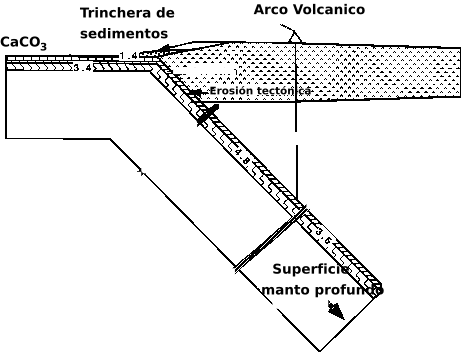
\includegraphics[width=0.6\textwidth]{tectonica.png}
 \caption[Ciclo del carbonato]{Representación del carbonato en la plataforma marina. Imagen modificada de \citep{sleep2001carbon}.}
  \label{fig:marc0.1}
\end{figure}


\subsection{Bomba biológica}

Si bien existe un ciclo del carbono que opera lentamente, también veremos a continuación un ciclo de carbono que funciona de forma paralela relacionado con los procesos biológicos, lo que hace que tenga escalas temporales más cortas y que esté directamente relacionado con la variabilidad climática \citep{sigman2003biological}. Así veremos la biogeoquímica que involucra la llamada \textit{bomba biológica}, en términos de los balances de carbono orgánico en el océano, sin considerar los ciclos y balances inorg\'anicos involucrados. \newpage

\begin{figure}[H]
\centering
 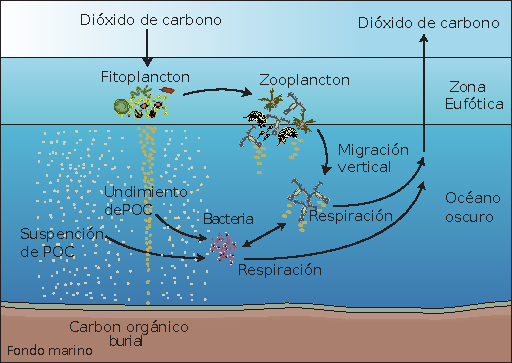
\includegraphics[width=0.9\textwidth]{pump.pdf}
 \caption[Modelo simple efecto bomba biológica]{Modelo simple efecto bomba biológica. La fijación fotosintética del carbono en la materia orgánica producida por el fitoplancton en la zona iluminada del océano (Carbono orgánico particulado, POC por sus siglas en inglés). Junto con la asimilación de macro y micro-nutrientes tales como, el nitrógeno, fosfato, hierro (principales limitantes) entre otros. Impulsa procesos de liberación de materia orgánica en esta capa, que son en su mayoría respirados y remineralizados. De la porción que logra escapar y se exporta al océano interior oscuro (zona afótica), una parte pequeña seguirá su camino hasta llegar a los sedimentos del fondo oceánico, mientras que la mayoría se remineralizará y oxidará a sus formas inorgánicas, gran parte de estas formas inorgánicas serán trasladadas de regreso a la zona eufótica producto de la circulación y mezcla, donde abastecerá de nutrientes a un nuevo crecimiento. Modificado de \citep{herndl2013microbial}.}
  \label{fig:bio1}
\end{figure} 

Producto de una diferencia en la presi\'on parcial del CO$_2$ gaseoso en la interfase oc\'eano-atm\'osfera y considerando que la presi\'on parcial de $CO_2$ tiende a estar en equilibrio, su aumento en la atm\'osfera fuerza un flujo hacia el oc\'eano. Cuando este gas entra en el océano, dentro de la gran variedad de ecosistemas que lo habitan, existen unos organismos llamados \textit{autótrofos}, que son aquellos que convierten este CO$_2$ en carbono orgánico. Esta conversión ocurre durante la \textit{fotosíntesis}, donde se utiliza como fuente de energía la luz solar, que mediante pigmentos, principalmente la clorofila, se transforma esta energía solar a energía química. La biomasa que realiza este proceso esta conformada mayormente por plancton en su forma bacterial (bacterioplancton), vegetal (fitoplancton) o animal (zooplancton) \citep{jeandelmarine}. Así el $CO_2$ entra en todos los constituyentes moleculares de estos organismo, en la forma

\begin{equation} \label{eq:marco1.2}
CO_{2} + H_{2}O + \textrm{energía solar} \rightleftharpoons CH_{2}O + O_{2}
\end{equation}

la fotosíntesis ocurre en la zona iluminada del océano (zona fótica), donde la profundidad de ésta capa de agua puede variar desde unos pocos metros (en zonas con alta turbulencia), hasta aproximadamente $150$ metros en aguas claras y con poca productividad. Además del carbono se requieren de otros macronutrientes para llevar a cabo la \textit{fotosíntesis}, tales como el nitrógeno (nitrato, NO$^{-}_{3}$), el fósforo (fosfato, PO$^{3-}_{4}$) y sulfato. Así la formación de la materia orgánica se puede ver

\begin{equation} \label{eq:marco1.3}
\begin{split}
106CO_{2} + 16HNO_{3} + 1H_{3}PO_{4} +122H_{2}O+ \textrm{energía solar} \rightleftharpoons \\
(CH_{2}O)_{106}(NH_{3})_{16}(H_{3}PO_{4})  + 138O_{2}
\end{split}
\end{equation}

Se aprecia la fijación de nitrógeno (NO$^{-}_{3}$) y CO$_2$ mediante la asimilación de ácido nítrico (HNO$_{3}$) para dar forma a los hidratos de carbono y aminoácidos (amonio), con la consecuente incorporación de fosfato para sintetizar las moléculas orgánicas. \\

La formación y productividad del fitoplancton estarán entonces relacionadas con la presencia u ausencia de carbono, nitrógeno y fosfato, en una proporción constante, que según \cite{redfield1934proportions} es C:N:P = 106/16/1. Sin embargo, a pesar de que el nitrógeno molecular (N$_2$) es muy abundante, existen pocos organismo que lo pueden absorber directamente, debido a que necesitan alta energía para lograr romper su triple enlace covalente, razón por la cual el balance entre la asimilación de N$_2$ a nitrógeno orgánico (fijación de nitrógeno) junto con la conversión de nitrato (desnitrificación) a N$_2$, son de vital importancia para el nitrógeno y para el inventario de nitrógeno biodisponible en la productividad marina. Por otro lado el PO$_{4}^{3-}$, es principalmente suministrado al océano por ríos, pero este aporte tiene mayor impacto en zonas costeras, en el océano abierto el suministro a la zona superficial deriva de procesos de surgencia o volcamiento oceánico, por ende, el PO$_{4}^{3-}$ utilizado por los organismos proviene mayormente de procesos de reciclaje. Así, muchas zonas del océano superficial tienen escasa o mínima concentración de NO$_{3}^{-}$ y PO$_{4}^{3-}$, que son consumidos completamente por el fitoplancton, lo que los hace los llamados elementos limitantes, es decir, que limitan el desarrollo del fitoplancton \citep{archer2000caused}. Entre estos también destaca el ácido silicio (Si(OH)$_4$) utilizado para construir los esqueletos de muchas especies de plancton, pero que es particularmente consumido por las diatomeas, un importante especie de fitoplancton responsable de gran parte de la producción de exportación de la tierra. Esta especie es menos propensa al consumo de fitoplancton por zooplancton (pastoreo), requiere de sílice en la forma de (Si(OH)$_4$) para el crecimiento y producción de sus frústulas (sílice biogénica, bSiO$_2$), lo cual luego será exportado en forma de sílice opalina \citep{treguer2000global,arellano2011high}. Además micronutrientes como el hierro (Fe) que será responsable de limitar la fijación de nitrógeno, dada su acción en la formación de la \textit{nitrogenasa} enzima del fitoplancton sintetizadora del nitrógeno molecular (N$_2$), una de las entradas más importantes de nitrógeno en regiones oligotróficas del océano \citep{mahaffey2005conundrum,gruber2008marine}. 

Por otro lado, el CO$_2$ que es asimilado por el fitoplancton está en su estado de carbono inorgánico disuelto (DIC), que se deriva de la reacción 

\begin{equation} \label{eq:marco1}
CO_{2 (g)} + H_{2}O\rightleftharpoons H_{2}CO_{3} \rightleftharpoons H^{+} + HCO_{3}^{-1} \rightleftharpoons 2H^{+} + CO_{3}^{-2} 
\end{equation}

El proceso qu\'imico que esta detr\'as de este mecanismo es el siguiente: el $CO_2$ cuando ingresa al agua de mar, se disuelve en el agua (producto de la temperatura y salinidad), reacciona con ella para formar \'acido carb\'onico $H_{2}CO_{3}$, pero este en general es inestable por ende tiende a liberar protones formando el i\'on carbonato de hidr\'ogeno $HCO_{3}^{-1}$ (bicarbonato) y el i\'on carbonato $CO_{3}^{-2}$ (carbonato), los que conjuntamente aumentan considerablemente la concentraci\'on de DIC en el agua\citep{Turekiangeochemistry}. El $CO_2$ como gas disuelto est\'a en muy peque\~nas cantidades, no alcanza el 2\% de la $\sum CO_2$ (suma de todas las concentraciones de las especies químicas del dióxido de carbono disuelto). La especie qu\'imica m\'as abundante en el oc\'eano es el bicarbonato, aproximadamente el 90\% del $CO_2$ que entra en el mar se encuentra en forma de i\'on bicarbonato y un $\sim$8\% en forma de i\'on carbonato. El $HCO_{3}^{-1}$ es m\'as consumido por procesos de fotos\'intesis que el CO$_2$ disuelto.

La materia orgánica que es producida por el fitoplancton, así como agregados de celular muertas, cuerpos de zooplancton o heces son consumida por bacterias heterótrofas y zooplancton.  Es rápida y generalizadamente remineralizada en la zona superficial, parte sin embargo, deja la zona eufótica para precipitarse hacia el océano profundo. No obstante, en esta lluvia de materia orgánica, esta materia es consumida por bacterias y animales, lo que hace que la materia se oxide y vuelva a sus componentes minerales, por esta razón, la concentración de nutrientes inorgánicos aumenta con la profundidad, a este proceso se le suele denominar ``respiración o remineralización'', alcanzando un máximo en torno a los 1000 metros de profundidad. 
Este proceso de consumo y liberación de nutrientes se puede ver como

\begin{equation} \label{eq:marco1.4}
\begin{split}
(CH_{2}O)_{106}(NH_{3})_{16}(H_{3}PO_{4})  + 138O_{2} \rightleftharpoons \\
106CO_{2} + 16HNO_{3} + 1H_{3}PO_{4} +122H_{2}O+ \textrm{energía química} 
\end{split}
\end{equation}

El nitrógeno, fosfato, DIC y hierro, siguen estas rutas como se puede apreciar en la figura \ref{fig:bio1}. Así, la remineralización ejerce procesos inversos en el océanos profundo. Por un lado, en ausencia de fotosíntesis, la concentración de nutrientes en su estado inorgánico aumentará en profundidad. Mientras que el carbono orgánico disuelto (DOC), o en su estados más pequeño particulado (POC) serán más altos en superficie y comenzarán a disminuir en profundidad. 

Finalmente, sólo el $1\%$  \citep{gruber2008marine} de la materia orgánica que logra alcanzar el lecho marino se almacena finalmente en los sedimentos del fondo oceánico (puede ser mayor en zonas costeras), y se reintegra al ciclo geológico del carbono. \newpage

\subsection{Volcamiento oceánico}

\begin{figure}[H]
\centering
 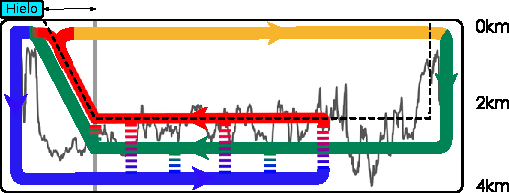
\includegraphics[width=0.7\textwidth]{ferrari2014antarctic.pdf}
 \caption[Circulación de volcamiento]{Circulación de volcamiento. La linea azul es la \textit{Agua Profunda de la Antártica}, la barra verde es la \textit{Agua profunda del Atlántico Norte}, la barra roja es el \textit{Agua Profunda de la India y del Pacífico} y la línea amarilla es la \textit{Agua Intermedia Antártica}. Imagen obtenida y modifica de \cite{ferrari2014antarctic}.}
  \label{fig:circ}
\end{figure}

La concentración de componentes inorgánicos almacenados en el océano profundo entre ellos el DIC, podrá volver a las aguas superficiales del océano por transporte de corrientes oceánicas o por procesos de surgencia. Este proceso de exposición de aguas profundas se da cada aproximadamente 1000 años \citep{sigman2000glacial}, donde el CO$_2$ ocasionalmente podr\'a ser liberada a la atm\'osfera, y los otros componentes reutilizados por la biolog\'ia. En este sentido, la \textit{circulación termohalina} (CTH) genera un transporte meridional de nutrientes y de DIC, que en procesos de ventilación oceánica, son importantes fuentes de carbono hacia la atmósfera \citep{toggweiler2006midlatitude}.  

La CTH es un gran transportado oceánico. La que ``comienza'' en la formación de aguas profundas en la zona del Atlántico norte (NADW) y en la Ant\'artica (AABW). Donde la NADW ser\'a desplazada en profundidad hacia el sur donde converger\'a con las aguas profundas y densas AABW, con las que producto de procesos de mezcla formará las aguas de la corriente Circumpolar profunda (CDW), las que llegará a superficie en la zona del Círculo Polar Antártico (ACC). Esta surgencia en superficie, estará siendo forzada por procesos de divergencia de aguas generado por los vientos del oeste. De esta manera, por transporte de Ekman la componente norte del afloramiento de aguas será trasladada a través de las termoclina de las distintas cuencas oceánicas (océano Índico, Pacífico y Atlántico) antes de retornar a la zona de hundimiento del océano Atlántico Norte (ver figura \ref{fig:circ}). Mientras, la componente sur del afloramiento de la CDW por diferencias de densidad, se hunde devuelta al océano profundo. 

A lo largo de este cinturón de corrientes se ve expuesta la actividad biológica. En zonas de surgencia o afloramiento oceánico se llevarán a superficie grandes contenidos de nutrientes inorgánicos, como el DIC, producido como vimos por procesos de remineralización y respiración en profundidad. Mientras, que en zonas de hundimiento o ``formación'' de aguas profundas, se verán secuestrados grandes contenidos de DIC producto de la utilización de nutrientes en superficie. 

 La CTH, no tan sólo es responsable del transporte de nutrientes por parte corrientes profundas y superficiales, si no además, es un gran transportador de calor en el océano. 

\subsection{Suministro de nutrientes}

En la producci\'on de materia org\'anica existen elementos que a menudo limitan la fotos\'intesis. Es usual hacer la distinci\'on entre macronutrientes (N y P) y micronutrientes 
(elementos traza) de acuerdo a su concentraci\'on relativa en los organismos. La concentraci\'on media de macronutrientes es del orden de los $mmol\ m^{-3}$ 
y la de los micronutrientes est\'a en el rango de los $\mu mol\ m^{-3} $ e inclusive m\'as baja (tal es el caso del hierro). Los elementos H, C y O son 
relativamente encontrados en abundancia y por ende, no son considerados como limitantes. 
De esta manera los organismos autótrofos que son los responsables de la fotos\'intesis en el oc\'eano toman estos elementos de la aguas superficiales
para formar materia org\'anica.  

Como vimos gran parte de la materia org\'anica es reciclada en superficie en ves de ser exportada. Así también, la mayor entrada de nutrientes es por suministros provenientes del oc\'eano profundo.
Debido al afloramiento por vuelco convectivo y de la mezcla vertical. Tambi\'en existe un transporte lateral donde la entrada de nutrientes proviene de la deposici\'on de la atm\'osfera, generalmente
es m\'as peque\~na pero puede ser localmente significativa. 

Sin embargo, este movimiento vertical en la columna de agua está asociado al estrés del viento en la superficie del océano, lo que induce un movimiento vertical que provocará una surgencia de nutrientes (giros ciclónicos) o de hundimiento de estos (giros anticiclónicos). Este movimiento vertical es conocido como el ``bombeo de Ekman''. Así la intensidad de la fotosíntesis estará directamente relacionada con la intensidad de este movimiento vertical. 

 De esta manera, al mismo tiempo que la diferencia del suministro de nutrientes crea ambientes distintivos que tienen un mayor impacto sobre los organismo que lo habitan, el suministro de luz ser\'a un factor determinante en la fijaci\'on de nutrientes inorg\'anicos disueltos (ver secci\'on 2.1.1). Donde la fuerte atenuaci\'on de esta en el agua de mar  incrementa r\'apidamente con profundidad, ocasionando que haya luz disponible para la fotos\'intesis s\'olo en las capas superficiales, cuya profundidad depende de la claridad del agua y de la cantidad de luz entrante (estaci\'on del a\~no). Este \'ultimo factor relacionado a la profundidad de la capa de mezcla, dado que si el grosor de la capa de mezcla es mayor que la zona euf\'otica, lo que normalmente ocurre durante invierno, los organismo fitoplanct\'onicos pasar\'an al menos parte de su tiempo en la oscuridad inclusive durante el d\'ia producto, por un lado, de la imposibilidad de controlar su posici\'on vertical, y por otro, a la mezcla vertical de la columna de agua. En tal caso, no hay suficiente luz para que su crecimiento exceda la respiraci\'on, por ende, si la capa de mezcla es suficientemente profunda pasar\'an mucho tiempo fuera de la zona euf\'otica y r\'apidamente morir\'an. Como consecuencia la supervivencia de concentraci\'on de nutrientes superficiales ser\'a alta, y el suministro de nutrientes y exportaci\'on de materia org\'anica ser\'an bajos.

Entonces clasificando los ambientes según su suministro de nutrientes y de luz tenemos: 

\begin{itemize}
 \item {\bf Zona ecuatorial (entre los 5$^\circ$N y 5$^\circ$S).} El constante suministro de luz como la surgencia ecuatorial que genera un transporte horizontal de corrientes fuera de la banda de surgencia (divergencia producida por los vientos alisios), hace que en esta zona los organismos microsc\'opicos del plancton sean muy productivos.

  \item {\bf Regiones subtropicales.} Regiones donde el giro anticiclónico de los vientos induce un hundimiento de las aguas superficiales, además no existe una estacionalidad marcada, por ende, la profundización de la capa de mezcla en invierno, hace que en conjunto el suministro de nutrientes a la capa superficial sea bajo durante todo el año (zona permanentemente estratificada). 
 
 \item {\bf Zonas subpolares.} Regiones donde la luz solar es interrumpida seg\'un la estaci\'on del a\~no y el giro ciclónico del viento induce una surgencia de aguas profundas aportando gran cantidad de nutrientes a la superficie, durante todo el año (un gran efecto de mezcla en invierno).

 \item{\bf Regiones costeras.} Tiene gran cantidad de suministro de nutrientes en los margenes este de las cuencas oceánicas debido al transporte de Ekman a lo largo de la costa.
\end{itemize}

Se han identificado zonas donde existe un alto potencial de suministro de nutrientes (alta surgencia) dado por el bombeo de Ekman y al mismo tiempo al buen suministro de luz, pero aún as\'i no poseen una bomba biol\'ogica eficiente debido a su limitación por hierro, el cual es esencial para una alta productividad y, por lo tanto, una fuerte bomba biol\'ogica,  estas son las llamadas zonas HNLC ``regiones con alto contenido de nutrientes, baja clorofila''. Las regiones HNLC incluyen los Océanos del Sur (incluyendo el margen hielo marino, giro subpolar, y subtr\'opicos estacionalmente estratificados), el Pacífico Ecuatorial y el Pacífico Norte (ver figura \ref{fig:Grilla4}). 

\section{Polvo/hierro y su impacto en el oc\'eano}

Datos obtenidos a partir de testigos de hielo de la Antártica, han mostrado que el CO$_2$ durante periodos glaciares e interglaciares, ha tenido una diferencia que va entre el rango de 80 - 100 ppm, con valores más altos durante periodos glaciares y más bajos durante interglaciares \citep{anderson2002southern,luthi2008high}. Por otro lado, estudios han mostrado que existe una alta correlación entre la temperatura y la concentración de CO$_2$ atmosférico, a la vez que también la temperatura a mostrado tener una buena correlación con los flujos de polvo durante periodos glaciares \citep{lambert2008dust}. \newpage

\begin{figure}[H]
\centering
 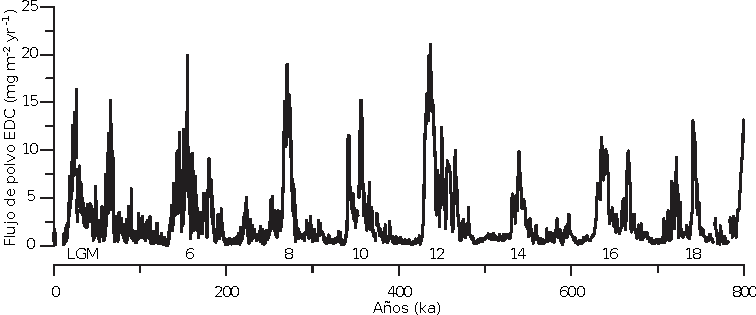
\includegraphics[width=0.9\textwidth]{lambert2008dust.pdf}
 \caption[Polvo en los últimos 800000 años]{Flujo de polvo, obtenido a partir del registro de \textit{EPICA Dome C} (EDC) de los últimos 800000 años. Imagen obtenida y modifica de \cite{lambert2008dust}.}
  \label{fig:dust}
\end{figure}

\cite{martin1990glacial} postula que el polvo mineral tiene un importante rol como fuente de micronutrientes para ciclos biogeoquímicos de la bomba biológica. 

\subsection{Polvo mineral}

\begin{figure}[H]
\centering
 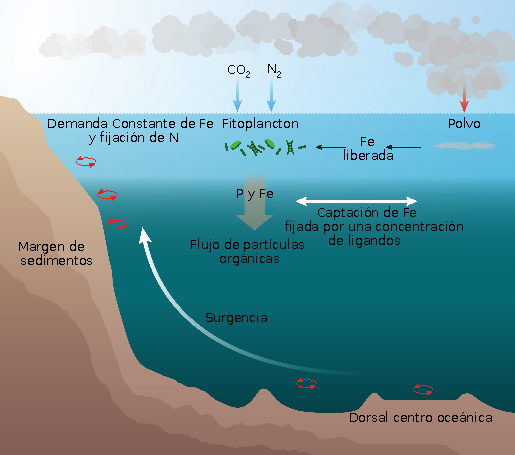
\includegraphics[width=0.75\textwidth]{dustt.pdf}
 \caption[Ciclo del hierro oceánico]{Esquema de la captación y funcionamiento del hierro en los océanos. Modificado de \citep{tagliabue2017integral}.}
  \label{fig:dust0}
\end{figure}

El polvo tiene un importante papel en la dinámica 
del clima, en el balance de energía, la microfísica de las nubes y en la química atmosférica \citep{tegen1994modeling,ridgwell2002dust,mahowald2011aerosol}. 

La erosión eólica en las regiones áridas y semiáridas, son las principales fuentes de flujos de polvo atmosférico (ver figura \ref{fig:dust4}). Esta erosión es una función directa de la velocidad del viento, siempre  y cuando se alcance un umbral que es definido como el límite sobre el cual las partículas comienzan a moverse por procesos de saltación. \cite{iversen1982saltation}, dicen que este umbral existe debido al peso de las partículas del suelo, es decir, que aumenta con el tamaño de grano y la fuerza de cohesión entre ellas que las mantienen sujetas a la superficie. No obstante, también la existencia de elementos no erosionables como la vegetación o rocas aumenta el umbral protegiendo el suelo y consumiendo parte del impulso del viento \citep{marticorena1997factors,tegen1994modeling} así también, la presencia de agua en el suelo aumenta la cohesión de las partículas producto del aumento de las fuerzas capilares entre ellas \citep{bopp2003dust} lo que sumado a la rugosidad, actúa absorbiendo una fracción de la intensidad eólica. De esta manera, la cizalle del viento, junto con el gradiente vertical de velocidad del viento se relacionan de la siguiente manera,

\begin{equation} \label{eq:marco1.5}
\begin{split}
\tau = \mu {\frac{\partial U}{\partial z}}
\end{split}
\end{equation}

Donde $U$ es la velocidad del viento, $z$ es la altura y $\mu$ es la viscosidad dinámica del aire. 

Una ves superado el umbral, los mecanismo que llevan a cabo este levantamiento de material, son: 1) arrastre aerodinámico que requiere de grandes velocidades de viento, 2) saltación, partículas que son lanzadas desde la superficie dibujando una trayectoria balística para impactar la superficie (tienen tamaños que van desde los 70 a 1000 $\mu$m) y 3) degradación de los granos producidos a partir del choque de partículas en la saltación (figura \ref{fig:dust2}). \newpage

\begin{figure}[H]
\centering
 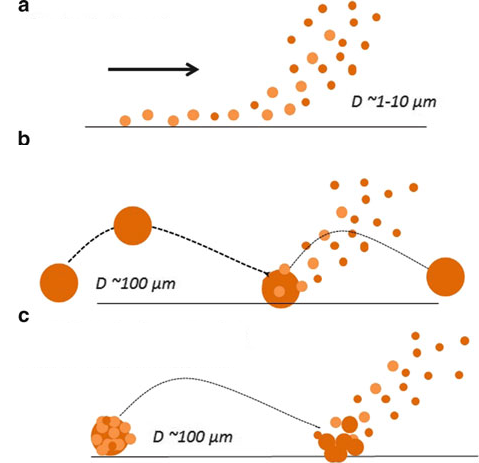
\includegraphics[width=0.5\textwidth]{dust2_pag97book.pdf}
 \caption[Mecanismos de emisión de polvo]{Mecanismos para la emisión de polvo, a) emisión aerodinámica, b) saltación por choque y c) degradación de fragmentos de agregados }
  \label{fig:dust2}
\end{figure}


De este movimiento de partículas sólo una fracción del orden 10$^{-6}$ se convertirá en un flujo vertical (polvo suspendido en la atmósfera) \citep{marticorena1997factors}. Finalmente la velocidad terminal dependerá tanto del peso de la partícula, la velocidad del viento, diámetro y densidad de la partícula, así como de las condiciones atmosféricas.

La generación de polvo es altamente variables según las condiciones locales. Así, entre los requisitos está, que la superficie del suelo esté seca y con poca vegetación, además deben haber altas concentraciones de partículas relativamente grandes (decenas a cientos de micr\'ometros de diámetro) para que el viento las pueda tomar y forzarlas a un movimiento. Esto generará rebotes a través de la superficie, que permitirá un desprendimiento de partículas más pequeñas (menos de 10 a 20 $\mu$m de diámetro) que pueden elevarse a la atmósfera, para recorrer grandes distancias como ``carga'' (ver figura \ref{fig:dust3}). Antes de ser depositadas mediante procesos de sedimentación gravitacional, turbulencia o de precipitación. \newpage

\begin{figure}[H]
\centering
 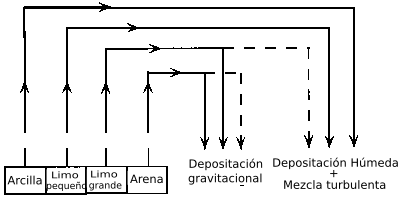
\includegraphics[width=0.65\textwidth]{depositacion.png}
 \caption[Esquema transporte de polvo]{Esquema de transporte de polvo \citep{tegen1994modeling} }
  \label{fig:dust3}
\end{figure}

\cite{prospero2002environmental} usando imágenes del satelitales desde 1978 hasta 1993, tuvo el propósito de identificar la distribución de las principales fuentes de polvo atmosférico, así termina definiendo el ``cinturón global de polvo'' que incluye África el Norte, Península Arabica, Asia Central, China, Australia, América del Norte, Sur África, y la zona sur de Sudamérica (Patagonia). 

\begin{figure}[H]
\centering
 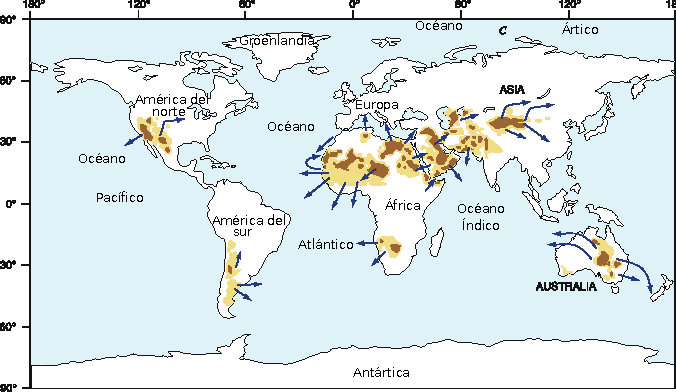
\includegraphics[width=0.9\textwidth]{dust4.pdf}
 \caption[Fuentes de polvo]{Distribución espacial de las fuentes de polvo globales, basada en múltiples imágenes satelitales. Las flechas azules indican las rutas de transporte de polvo \citep{muhs2014identifying}.}
  \label{fig:dust4}
\end{figure} 

Por otro lado, la caracterización mineral del polvo muestra que  el Si es el componente más abundante. Sin embargo, proporciones de Ca, Mg y Fe tienen una diferenciación dependiendo de la fuente. Mientras que elementos como K, Na, Fe, Mn, Ti, P, muestran una distribución mas menos constante \citep{scheuvens2013bulk}. 

Así vemos que el polvo puede llevar consigo nutrientes, los que eventualmente podrían transportarse a grandes distancias. Una de las consecuencias es que puede suministrar fósforo y hierro a ecosistemas terrestres y marinos, lo que modificará los ciclos de productividad de regiones que se encuentran cerca y lejos de las fuentes de polvo \citep{martin1990glacial,anderson2002southern,lambert2015dust,bopp2003dust} (ver figura \ref{fig:dust0}). 

Como se vio en la sección anterior existen zonas oceánicas que están limitadas por hierro (zonas HNLC) o también por fosfato  (giros subtropicales), sin embargo, y a pesar de que el hierro es el cuarto elemento más abundante en las rocas continentales, tiene una muy baja solubilidad (Fe$^{3+}$) \citep{archer2000caused}, que bajo la presencia del oxígeno molecular O$_2$ es rápidamente oxidado de su estado Fe$^{+2}$ (más soluble) en la superficie del océano \citep{martin1990glacial}, así las concentraciones de hierro soluble son cercanas a 1 nmol$^-1$. Del hierro suministrado por el polvo atmosférico, sólo alrededor del $10\%$, está disponible para ser absorbido por el fitoplancton (Fe$^{+2}$). 

En el agua el hierro se encuentra en su forma más oxidada debido a la reacción: 

\begin{equation} \label{eq:marco2.1}
Fe^{3+} + 3OH^{-} \rightleftharpoons Fe(OH)_{3 \textrm{sólido}}
\end{equation}

Por esta razón es que muchos organismo marinos (algas), han desarrollado 
mecanismos para la formación de ligandos \textit{sideroforos}, moléculas que disuelve el ion hierro Fe$^{3+}$ a complejos Fe$^{2+}$ \citep{martin1990glacial,tagliabue2017integral}. Estos ligandos normalmente están unidos a la membrana celular y presentar una gran afinidad por metales traza que transportan. Para el caso del hierro, existen dos tipos de ligandos transportadores, activos los que son producidos por bacterias marinas heterótrofas, hongos y fitoplancton dinoflagelado. Se desarrollan bajo condiciones de limitación del crecimiento, emitiéndose al medio acuático donde reaccionan con el hierro, formando complejos que penetran nuevamente en los organismos, mediante un transporte activo en las proteínas de membrana.
Debido a la alta afinidad de los sideróforos con el hierro Fe$^{3+}$, en condiciones de menor concentración que el hierro se encuentra completamente unidos al metal. 

Por lo tanto, dentro del oc\'eano el hierro esta fusionado org\'anicamente 
y siendo constantemente reutilizado teniendo un tiempo de residencia de unos meses a años \citep{boyd2010biogeochemical}.

La limitaci\'on de hierro en aguas superficiales refleja concentraciones que son inadecuadas para la formaci\'on de fitoplancton debido a que la regeneraci\'on de \'este es m\'as lenta que el 
hundimiento de hierro contenido en materia org\'anica. As\'i para el mantenimiento de la producci\'on primaria del oc\'eano abierto se requiere un aporte mayor que el dado por el afloramiento, el cual generalmente es atmosf\'erico.

As\'i la absorci\'on de hierro por algunos fitoplancton hacen que este influya en la comunidad de algas, y por tanto, en la productividad en general. Cabe destacar que el fitoplancton de mar abierto 
por lo general requiere de menos hierro que las especies costeras, las que se han desarrollado en un ambiente rico en hierro. As\'i se ha logrado un requerimiento menor de hierro reduciendo el tama\~no
de las c\'elulas y minimizando el n\'umero de enzimas que contienen hierro \citep{palenik2003genome}. Sin el estr\'es de hierro veremos presencia de fitoplancton con c\'elulas m\'as grandes. 

Aparte de la limitaci\'on directa de la
producci\'on primaria en las zonas HNLC el hierro puede limitar la fijaci\'on de nitr\'ogeno de las especies fotosint\'eticas. 

En las regiones HNLC los cambios en el suministro de hierro afectar\'an directamente la producci\'on primaria y la composici\'on de las especies, mientras que en las regiones oligotr\'oficas
subtropicales/tropicales el impacto ser\'a principalmente a trav\'es de cambios en la fijaci\'on de nitr\'ogeno \citep{jickells2005global}. 

Por otro lado, dado que la solubilidad del hierro es baja se estima que hay grandes concentraciones de part\'iculas de hierro en el onc\'eano profundo, de esta manera si parte de este polvo se disuelve en profundidad aumentar\'an las concentraciones abisales de hierro disuelto, y a largo plazo la productividad en las regiones de surgencia como 
los oc\'eanos del sur \citep{parekh2005decoupling}. 

\section{Última deglaciación}

El Pleistoceno se ha caracterizado por ciclos glaciares/interglaciares que han tenido terminaciones abruptas, donde llegan a un máximo interglacial que generalmente ocurre al comienzo del interglacial, luego se produce un descenso de las temperaturas para comenzar una glaciación, posteriormente las temperaturas descienden hacia un máximo glacial. Se sabe que estos periodos han estado sujetos a variaciones relacionadas con parámetros orbitales de la Tierra denominados ``ciclos de Milanckovitch'', que tienen periodos de 100, 41 y 23 mil años, donde particularmente los últimos 800 mil años han tenido una periodicidad de 100 ka. 

\begin{figure}[H]
\centering
 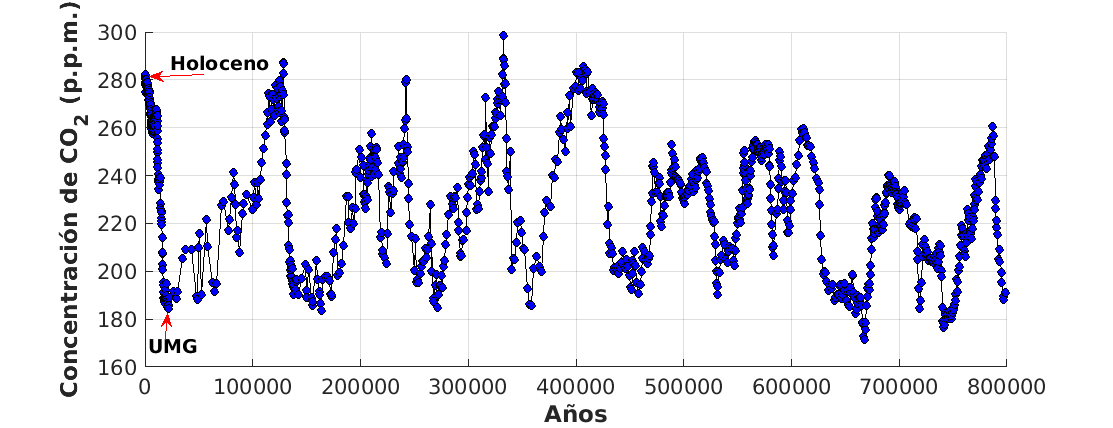
\includegraphics[width=1\textwidth]{CO2glob.png}
 \caption[Registro de CO$_2$, últimos 800 mil años]{Registro de CO$_2$ de los últimos 800000 mil años. Datos obtenidos de \citep{luthi2008high}. }
  \label{fig:CO2}
\end{figure}

La última deglaciación corresponde a la transición entre el periodo de máximo estadial del último ciclo del cuaternario (ocurrido aproximadamente hace 21000 años a.p.) \citep{clark2009last}, conocido como el Último Máximo Glacial (UMG), y el comienzo del Holoceno (\string~ 12000 años  a.p.) \citep{sigman2000glacial,barker2009interhemispheric}.


\subsection{\'Ultimo m\'aximo glacial}
 
 El UMG es el periodo más frío dentro del último periodo glacial correspondiendo al rango de tiempo desde 26.5 ka a 21 ka \citep{clark2009last}. Gracias a diversos paleoproxies, es sabido que durante este periodo 
las concentraciones de pCO$_2$ fueron cercanas a las 180 partes por millón por volumen (p.p.m.v) \citep{luthi2008high}, habían bajas temperaturas, el nivel del mar era 120 m. más bajo que el nivel
 actual \citep{fairbanks198917,denton2010last,lambeck2014sea} debido a una gran expansión de los casquetes de hielo polar como es el caso de Laurentide en el Hemisferio Norte que fue creciendo desde el comienzo de la última glaciación hasta alcanzar su máxima extensión en el UMG \citep{fairbanks198917}, y el océano global era 3\% más salado que en la actualidad \citep{sigman2000glacial,bopp2003dust}. Además diversos modelos y registros paleoclimáticos han mostrado que habían mayores flujos de polvo, debido a posibles aumentos del área de las fuentes, y/o por intensificación de los vientos o disminución del ciclo hidrológico \citep{mahowald1999dust,lambert2008dust,maher2010global}. 

\begin{figure}[H]
\centering
 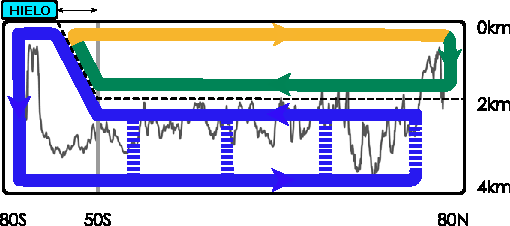
\includegraphics[width=0.6\textwidth]{LGMWater.pdf}
 \caption[Circulación de volcamieno en el LGM]{\textit{Circulación de volcamieno en el LGM.} La linea azul es el agua proveniente de la Antártica que llena las profundidades abisales e intermedias del océano, mientras la barra verde es el agua del Atlántico Norte que llegaba a profundidades intermedias, y la linea amarilla es la Agua Intermedia Antártica. Imagen obtenida y modifica de \citep{ferrari2014antarctic}.  } 
\label{fig:aguaCO2}
\end{figure}

 Por otro lado, la circulación oceánica durante este periodo se cree fue más estratificada (ver figura \ref{fig:aguaCO2}) \citep{sigman2000glacial,lynch2007atlantic,tagliabue2009quantifying,ferrari2014antarctic}. Una de las teorías de esta mayor estratificación es debido al carácter estacional de la formación de capa de hielo del Hemisferio Norte (en invierno se crea volumen de hielo y en verano el agua se refresca por derretimiento). Esto según \cite{ferrari2014antarctic}, habría producido durante el UMG un resfrescamiento del agua en el Atlántico Norte, lo que produciría que las aguas superficiales provenientes de las zonas ecuatoriales no lograran niveles de densidad suficiente para producir un volcamiento adecuado, por esta razón las formación de aguas del Atlántico Norte no habrían superado profundidades mayores a 2 km. Así se dice que durante el UMG el volumen oceánico fue llenado por aguas de origen Antártico. No se habría producido la \textit{Agua Profunda Circumpolar} (CDW) por lo tanto los regímenes no habrían mantenido contacto producto de mezcla vertical. Otro teoría es propuesta por \cite{toggweiler2006midlatitude}, que se refiere a un debilitamiento de la CDW como resultado de un movimiento hacia el ecuador de los \textit{vientos del oeste} durante periodos glaciares, lo que conduciría a menor divergencia de agua superficial, por lo tanto, a menor surgencia de agua profunda. 

 Además, el volumen de hielo marino se habría expandido hasta el \textit{Frente Polar Antártico} durante invierno, y a niveles cercanos a los actuales durante el verano \citep{bopp2003dust}. Esto tienen particular importancia en los Océanos del Sur dado que es en esta zona donde se refrescan las aguas densas, con mucho contenido de CO$_2$ (producto de la respiración oceánica) y nutrientes provenientes del océano Atlántico, Indico y Pacifico (ver sección Bomba Biológica). Por esta razón, un aumento de la cobertura de hielo de la zona Antártica, habría generado un bloqueo de gran parte de la surgencia de agua profunda, afectando de esta manera tanto la liberación de CO$_2$ como, los ciclos biogeoquímicos del océanos. 

\subsection{Terminación I}

Como se mencionó y se puede apreciar en la figura \ref{fig:CO2}, todos los ciclos glaciares han finalizado por un abrupto cambio desde un estado de máxima glaciación a un estado de rápidos incrementos de temperatura. La última transición Glaciar-Interglacial no es la excepción a esta regla. 

La terminación I, comenzó hace aproximadamente 21000 años atrás en el Hemisferio Norte, y hace aproximadamente 18000 años atrás en el hemisferio Sur \citep{denton2010last,clark2009last,lynch2007atlantic}.  Lo anterior debido al comportamiento dipolar entre los hemisferios, finalizando aproximadamente hace 12000 años atrás. 

\cite{denton2010last}, propuso una serie de factores que a su juicio podrían haber gatillo el comienzo de este periodo de transición. Todo comienza con un aumento de la insolación de verano en el Hemisferio Norte (H.N), sin embargo, esto es insuficiente para explicar la rápida y gran variación. Así lo anterior, en conjunto con una gran extención de la cubierta de hielo del Hemisferio Norte, habría generado una presión isostática del hielo que no fue posible mantener provocando grandes eyecciones de flujos de hielo y agua dulce producto del derretimiento y la ablación, a zonas de hundimiento de agua en el Atlántico Norte, afectando la circulación de volcamiento \citep{ferrari2014antarctic}. Producto de cambios de temperaturas del agua superficial, la zona de \textit{interconvergencia intertropical}
fue desplazada hacia el sur. Mientras tanto, el Hemisferio Sur que se mantenía en sus condiciones glaciales, en la zona Antártica se comenzaron a derretir los casquetes de hielo producto de un desplazamiento de los vientos del oeste hacia los polos, incrementando la surgencia en la \textit{Corriente Circumpolar Antártica} (ACC) lo que produjo una liberación de CO$_2$, que habría amplificado el efecto de incremento de temperaturas medias. 

Sin embargo, este periodo no estuvo exento de variaciones climáticas tanto en el H.N. como en el H.S. además de la evidencia que se ha mostrado acerca de la asincronía interhemisférica lo que se ha denominado el ``balancín dipolar''. Así, luego de dar comienzo a la Terminación I en el H.N. registros han mostrado un enfriamiento en el Atlántico Norte, conocido como \textit{Heinrich estadial 1} (HS1), mientras en el mismo lapsus de tiempo en el Hemisferio Sur significó el comienzo de la transición. El mismo efecto es visto por la llamada \textit{Reversión fría Antártica} (ACR) en el H.S. lo que en el H.N. se ve reflejado como un periodo cálido denominado intervalo \textit{Bølling–Allerød} ($\sim 14.7$ mi años) \citep{renssen2001two}, luego en el Hemisferio Norte hay evidencia de un nuevo periodo frió conocido como \textit{Younger Dryas} ($\sim 12.8–11.5$ mil años) lo que implicó la completa deglaciación del H.S. \citep{denton2010last,barker2009interhemispheric}.

\subsection{Holoceno}

Así se llegaría entonces al fin del periodo Cuaternario y comienzo del Holoceno, con una concentración atmosférica de CO$_2$ en torno a las 280 p.p.m. \citep{sigman2000glacial}. Pero que desde el periodo preindustrial, ha ido en aumento.

 Esta época al igual que la Terminación I se ha caracteriza por una marcada inestabilidad. Con una fuerte relación con la irradiansa solar, generando ``ciclos'' con una periodicidad promedio de 1500 años en el Hemisferio Norte \citep{bond2001persistent}. Afectando la posición de la \textit{Zona de Interconvergencia Tropical} (ITCZ) \citep{haug2001southward}, y la posición e intensidad de los vientos del oeste \citep{moreno2010covariability,lamy2010holocene}. Así en periodos con una baja irradiansa solar, en el Hemisferio Norte hay registros de grandes apariciones de hielo a la deriva, enfriando el océano superficial y la temperatura atmosférica de Groenlandia, lo que se traduce en una reducción de la precipitación en latitudes medias \citep{bond2001persistent}. 

 Respecto de la fuentes y niveles de polvo atmosférico, éstos tienen una notable disminución, como tanto los registros como los modelos muestran (ver sección 4.1) \citep{mahowald1999dust,kohfeld2001dirtmap} debido presumiblemente, a la disminución de la intensidad de los vientos.

\section{Modelos}

\begin{figure}[H]
\centering
 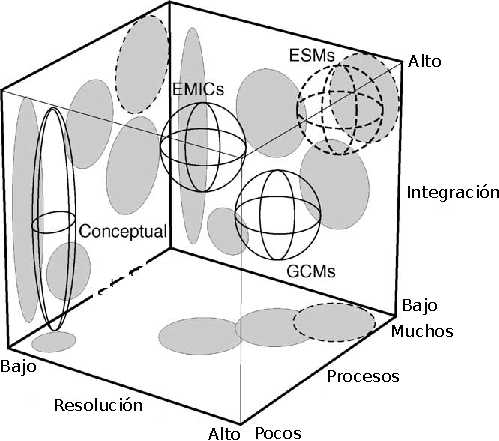
\includegraphics[width=0.5\textwidth]{modelos2.pdf}
 \caption[Tipos de modelos]{Grado de complejización de los modelos, en función de su nivel de resolución y procesos que incluyen. El modelo en línea punteada corresponde a los \textit{Modelos de Sistema Tierra}. Figura adaptada de \citep{bartlein2003modeling}. }
  \label{fig:modelos}
\end{figure}

El sistema climático se considera formado por componentes que tienen características bioticas y abioticas, tal como, la geósfera que incluye la atmósfera, hidrósfera (principalmente ríos y océanos), la criósfera (hielo marino, permafrost, hielo interior y cubierta de nieve), la pedósfera (suelo) y la litosfera (corteza terrestre y manto superior de la Tierra), sistemas abiertos que en conjunto son conocidos como el sistema climático físico, que interaccionan con la componente biosférica. 

Con el desarrollo de la ciencia computacional, el progreso de la termodinámica en los años 90s y el creciente interés por entender los procesos que gobiernan la variabilidad climática es que se sentaron las primeras bases de los principios físicos que gobiernan el flujo atmosférico \citep{lynch2008origins}.  Con ello se dio paso desde los modelos conceptuales a los modelos más complejos que integraban las atmósfera y el océano (ESM, \textit{Modelos del Sistema Tierra}) \citep{flato:hal-01644494}. 

Los tipos de modelos se diferencias en su grado de complejidad, es decir, el grado de componentes que posee y utiliza para reproducir el sistema Tierra \citep{weber2010utility}.

 Los modelos conceptuales están basados en conceptos del funcionamiento del sistema Tierra, diseñados para ser computacionalmente eficientes. Entre estos destacan los \textit{Modelos de Balance Energéticos} (EBMs, por sus siglas en inglés) y los modelos de caja. Los primeros, resuelven el balance de calor radiativo de la atmósfera en términos de la temperatura superficial del aire. Existen en una y dos dimensiones. Otros, son los modelos de caja, modelos simples con baja resolución espacial cuyas cajas son representaciones de relaciones biogeoquímicas, que sacrifican el grado de realismo físico pero dan una exploración de los parámetros espaciales en cuestión.

  Por otro lado, se encuentran los modelos más complejos \textit{Modelos de Circulación General} (GCM, por sus siglas en ingles), pero menos integrados que se enfocan en la dinámica atmosférica y del océano. Son modelos que resuelven la ecuación fundamental de movimiento, junto con la evolución de la temperatura y humedad de la atmósfera o la temperatura y salinidad de los océanos. Contienen una baja cantidad de componentes que son directamente acopladas. Estos modelos son más realistas, pero poseen un alto costo computacional, por lo que son usados mayormente para experimentos multidecadales, aunque tambi\'en para an\'alisis del tiempo sin\'optico un subconjunto conocido como \textit{Modelos Climáticos Regionales.} Los \textit{Modelos de Sistema Tierra de Complejidad Intermedia} (EMICs, por su sigla en inglés), es un tipo de modelo acoplado (lo que permite escoger los m\'odulos que se desean simular en funci\'on de la pregunta que se plantea), que se encuentra en el medio de los dos comentados anteriormente (ver figura \ref{fig:modelos}), estos describen el sistema climático con menos detalle espacial y temporal que los GCMs, con mayor simplicidad de sus componentes físicas, pero incluyen más procesos integrados de forma parametrizada, lo que permite una mayor interacción de los módulos al representar procesos y un bajo costo computacional (ver tabla \ref{tabla:modelos}), a la vez que tambi\'en pueden integran balances biogeoquímicos \citep{claussen2002earth,flato2011earth}. Además se diferencia de los modelos conceptuales dado que sus grados de libertad exceden (por mucho) las parametrizaciones que posee \citep{weber2010utility}. Los EMICs, fueron diseñados para reproducir escalas de tiempo que están entre 10$^2$ y 10$^5$ años. Permiten hacer simulaciones de sensibilidad. Finalmente, los \textit{Modelos de Sistema Tierra} (ESMs, por su sigla en ingl\'es), son modelos acoplados interactivamente que integran tanto las din\'amicas de la circulaci\'on vistas en los GCMs como las caracter\'isticas que son manejadas por los EMICs, siendo un modelo altamente integrado pero que se caracterizan adem\'as, por una alta resoluci\'on espacial aunque computacionalmente limitados \citep{bartlein2003modeling}. 


\begin{table}[H] 
\centering
\resizebox{12cm}{!} {%
\begin{tabular}{|cc|}
\hline \hline
\multicolumn{2}{c}{\bf Parametrización} \\
%\cline{2}
\hline \hline
Componentes & Características  \\
\hline \hline
\multirow{3}{*}{Atmósfera}  & Convección y microfísica de nubes  \\ \cline{2-2}
& Aerosol e interacciones \\ \cline{2-2}
& Capa límite \\ \cline{2-2}
& Radiación \\ \hline
Océano& Difusión y advección de remolinos \\ \hline
\multirow{2}{*}{Tierra} & Vegetación/Tipo de suelo \\ \cline{2-2}
& Humedad \\ \cline{2-2}
& Nieve o agua subterránea \\ \hline
Cubierta de hielo & Propiedades dinámicas y termodinámicas \\ \hline
\multirow{4}{*}{ * Ciclo de carbono} & Procesos químicos y biogeoquímicos \\ \cline{2-2}
& Captación de CO$_2$ \\ \cline{2-2}
& Especies de plancton y fitoplancton \\ \cline{2-2}
& Inclusión de carbonato de calcio (CaCO$_3$) \\ \cline{2-2}
& Partículas de aerosol\\ \hline
\multirow{2}{*}{ * Partículas de aerosol} & Ciclo de azufre \\\cline{2-2}
& Efecto directo e indirecto del aerosol de sulfato \\ \cline{2-2}
& Polvo en aerosol \\ \hline 
\multirow{1}{*}{ * Ciclo de metano y permafrost} & Química atmosférica del CH$_4$ \\ \cline{2-2}
& Emisiones de CH$_4$ en humedales \\ \hline
\multirow{2}{*}{ \makecell{* Dinámica global de la vegetación\\ e incendios forestales}} & \makecell{hidrología del suelo \\ (superficial y subsuperficial)} \\ \cline{2-2}
& descarga de agua en ríos \\ \cline{2-2}
& Intercambio de agua con la atmósfera \\ \cline{2-2}
& Fuentes ecológicas \\ \cline{2-2}
&  \makecell{Interacción del ciclo del carbono \\ inclusión de Gases trasas CH$_4$, N$_2$O y NO$_X$} \\ \hline
* Uso y cambio de suelo & \makecell{Tratamientos de cultivos \\ e interacción con el paisaje y zonas urbanas}\\ \hline
\multirow{2}{*}{\makecell{ * Interacciones químicas del clima y \\ acoplamiento estratosférico - troposférico}} & Circulación troposférica \\ \cline{2-2}
& Dinámica estratosférica \\ \cline{2-2}
& Interacción dinámica estratosférica - troposférica \\ \hline
* Capas de hielo en la tierra & \makecell{Tasa de agua derretida provenientes \\ de la Antártica y Groenlandia} \\ \hline
\multirow{3}{*}{\makecell{* Características adicionales \\ acoplamiento Océano-Atmósfera}} & Corrientes oceánicas superficiales \\ \cline{2-2}
& Radiación solar que penetra en el océano \\ \cline{2-2}
& Captura de radiación por la clorofila \\ \cline{2-2}
& Distribución de clorofila \\ \hline \hline
\end{tabular}%
}
\caption[Componentes de modelos]{Componentes de los modelos GCMs y EMICs. Los marcados con asterisco son los que sólo se incluyen en los modelos EMICs y ESM. } 
\label{tabla:modelos}
\end{table} 


\chapter{\'Area de Estudio}

% !TEX root = ../Tesis_NataliaOpazo.tex

El \'area de estudio comprende la totalidad del globo (figura \ref{fig:Grilla4}). Se ver\'a con especial atenci\'on zonas regionales del oc\'eano (HNLC) que se encuentran definidas en la tabla \ref{tabla:Area1} y que gr\'aficamente podemos apreciar en la imagen
\ref{fig:Grilla4}. 

\begin{figure}[H]
\centering
  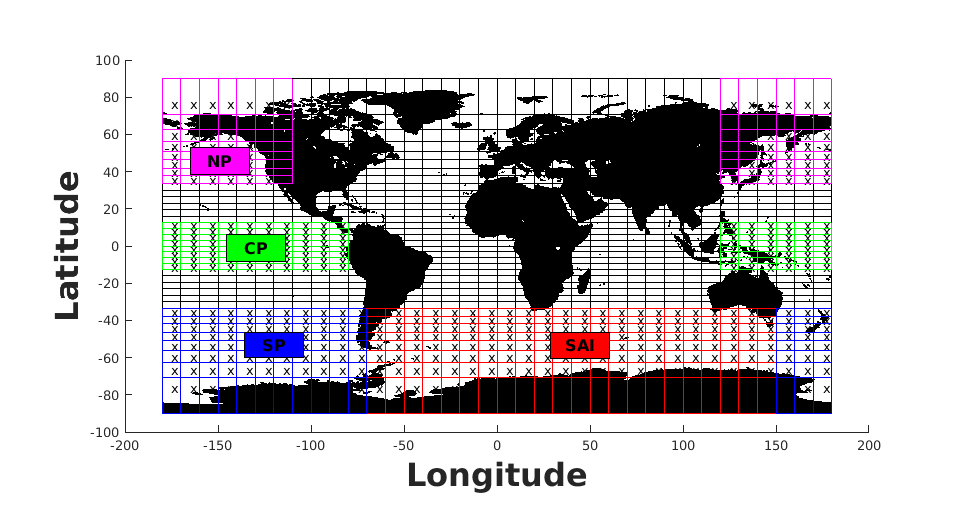
\includegraphics[width=0.9\textwidth]{mapa.png}
  \caption[Grilla global y regional de campos de flujo de polvo]{Grilla cGenie con la especificaci\'on de las zonas HNLC a simular: Pac\'ifico norte (NP), Pac\'ifico Sur (SP), P\'acifico Central (CP) y Atl\'antico/Índico Sur (SAI).}
  \label{fig:Grilla4}
\end{figure} 

El detalle de las distintas regiones oce\'anicas se presentan en la tabla a continuaci\'on. \newpage

\begin{table}[H]
\begin{center}
\begin{tabular}{l|l|l|l|l}
\hline
\multirow{2}{1cm}{ Zona}& Latitud & Longitud &Puntos & \'Area \\
 & cuadrante & cuadrante & de grilla & total  ($km^{2}$)\\
\hline \hline
Atlántico/Índico del Sur (SAI)& -90 a -33.7490 & -70 a 150 & 176&  6.9268e+07 \\ \hline
Pac\'ifico Sur (SP) & -90 a -33.7490 & -180 a -70 y 150 a 180& 112 & 4.4080e+07  \\ \hline
Pac\'ifico Norte (NP) & 33.7490 a 90 &  -180 a -110 y 120 a 180 & 104 & 4.0931e+07\\ \hline
Pac\'ifico Central (CP) & -12.8396 a 12.8396 & -180 a -80 y 120 a 180 & 128 & 5.0377e+07 \\ \hline
\end{tabular}
\caption{Caracter\'isticas de las regiones oce\'anicas simuladas en cGENIE.}
\label{tabla:Area1}
\end{center}
\end{table}


\chapter{Metodolog\'ia}

% !TEX root = ../Tesis_NataliaOpazo.tex

 A continuación se presenta la estructura de este trabajo para comprender la interacción entre la productividad biológica, la biogeoquímica y el clima. Se utilizó para ello un modelo del ciclo del carbono con una representación del ciclo biogeoquímico del océano, durante el periodo correspondiente a la transición del Pleistoceno al Holoceno. Para lo cual se presentan los flujos de campo de polvo, provenientes tanto de reconstrucciones como de modelos simulados. El trabajo estará enfocado en cuantificar los efectos del ciclo biogeoquímico del hierro en la bomba de tejidos blandos, relacionándolo con la captura del CO$_2$ tanto a global como en las zonas HNLC. 

 Para poder responder al objetivo general, este trabajo seguirá la siguiente estructura: 

\begin{itemize}
\item[\bf I.] Tratamiento del modelo cGENIE al ciclo del hierro oceánico (sección 4.1).
\item[\bf II.] Se presenta la fuente de los datos (sección 4.2). Las que nos describen la cantidad de fuentes de polvo en ambos periodos UMG y Holoceno.  
\item[\bf III.] Pre-procesamiento de los datos (sección 4.3). Se editan las fuentes de polvo con el objeto de dejarlas como input para el modelo cGENIE. 
\item[\bf IIII.] Procesamiento (sección 4.4). Se simulan las fuentes de polvo con el propósito de ver el efecto del hierro en la captura de CO$_2$. 
\end{itemize} \newpage

 \section{Modelo cGENIE}
En este estudio se utilizó un código versión ``muffin'' del \textit{cGENIE Earth system Model of Intermediate Complexity}, en su versión 0.9 (genie.seao2.or). Este modelo fue construido a partir del \textit{Grid ENabled Integrated Earth system model} GENIE, siendo una simplificada versión centrada en el ciclo del carbono \citep{ridgwell2007marine}. En este estudio se usa una versión GENIE que contiene una atmósfera simplificada y que se encuentra centrada en el ciclo del carbono, conocida como cGENIE. Utilizada comúnmente para conocer las interacciones entre la productividad biológica, la biogeoquímica y el clima. Como todo EMIC, este modelo contiene distintas componentes del sistema Tierra. Incorpora representación de la circulación oceánica, biogeoquímica marina, sedimentos del fondo marino y geoquímica \citep{lenton2007effects}. No obstante, el modelo tiene una baja resolución espacial, y una discreta resolución temporal realizando simulaciones de una escala entre 10$^4$ y 10$^5$ años \citep{meyer2016influence} relevante para procesos de retroalimentación biogeoquímica, lo que hace que sea extremadamente eficiente \citep{edwards2005uncertainties}. 

El modelo GENIE-1 contiene 49 trazadores disueltos, propiedades isotópicas importantes en un contexto de cambio climático y estudios paleo, y relaciones molares (si las hay) en sedimentos sólidos y gases atmosféricos. El presente modelo es utilizado con el prop\'osito de conocer los escenarios pasados de pCO$_2$ atmosf\'erico, basado en el impacto de la fertilizaci\'on con hierro procedente de los flujos de polvo a\'ereos en la ecolog\'ia marina. Es por esta razón, que se define el uso de los siguientes trazadores atmosféricos: CO$_2$, $^{13}$C, O$_2$, con la adición de la temperatura y humedad de la atmósfera. Mientras que para el océano: carbono inorgánico total disuelto (DIC), alcalinidad (ALK), fosfato (PO$_4$), hierro (Fe), Oxígeno (O$_2$), las componentes de carbono, fósforo y hierro de materia orgánica disuelta, isótopos estables ($^{13}$C) asociadas al DIC y al DOM, ligandos limitados por hierro, ligandos libres (que pueden enlazarse con hierro). 

Se calcula la redistribución de la concentración de trazadores que no son transportados debido a la circulación oceánica. Así, se ve que la remoción de la solución de nutrientes (PO$_4$ y Fe), el DIC y al alkalinidad, entre otros, ocurre mediante la captación por la productividad biológica en la zona eufótica del océano. Habrá entonces una exportación resultante de material particulado que dependerá de los procesos de remineralización, que eventualmente podrían constituir una nueva solución inorgánica, pero esta vez, a mayor profundidad en comparación de donde los trazadores fueron retirados originalmente. 

Los módulos utilizados para llevar este proceso a cabo son: 

\begin{table}[H]
\centering
\begin{tabular}{|l|l|l|}
\hline
Componente& Abreviatura & Modelo \\
\hline \hline
Atmósfera & eb& EMBM (2-D) \\ \hline
Océano & go & GOLDSTEIN \\ \hline
Cubierta de hielo oceánica &gs& GOLDSTEIN (opciones multiples)  \\ \hline
Química atmosférica&ac&ATCHEM\\\hline
Biogeoquímica oceánica&bg&BIOGEM\\ \hline
\end{tabular}
\caption[Componentes modelo cGENIE]{Detalle de los modelos utilizados y las cacacter\'isticas asociadas a los campos de hierro globales}
\label{tabla:Met1}
\end{table}

\begin{description}

\item{\bf C-GOLDSTEIN}

Módulo que contiene la componente climática y de la física oceánica. Entre sus características incluye una fricción geostrófica reducida, un modelo 3-D de circulación oceánica acoplada, un modelo 2-D de balance de energía-humedad de la atmósfera (EMBM) y un modelo de dinámica-termodinámica del hielo marino \citep{edwards2005uncertainties}.

\item{\bf BIOGEM (BIOGEochemical Model)}

Modulo que se encuentra compuesto y maneja el intercambio gaseoso océano-atmósfera, y la transformación y redistribución espacial de los componentes biogeoquímicos tanto en la superficie (captura biológica) como en el interior del océano (remineralización) \citep{ridgwell2007regulation}. 

\end{description}

 \section{Base de datos}

Entre la base de datos utilizadas se encuentra una reconstrucción y cuatro modelos de polvo (ver secci\'on 2.2) para el periodo del Último Máximo Glacial y el periodo preindustrial. 

A continuaci\'on se presentan la reconstrucci\'on y modelos utilizados.

\subsection{Reconstrucción}

 {\bf Lambert.} Los flujos de depositación de polvo presentados a continuación, corresponden a una reconstrucción basada en datos obtenidos del \textit{Dust Indicators and Records of Terrestrial and Marine Paleoenvironments} (DIRTMAP) en su tercera fase. DIRTMAP es un registro de datos geológicos compilados en la forma de un set de datos espacializados \citep{kohfeld2001dirtmap}, creados con el fin de servir como evaluación para simulaciones desarrolladas con modelos del sistema Tierra que incluyan una componente del ciclo de polvo. 

Esta base de datos fue previamente seleccionada por \cite{lambert2015dust}, que extrajo dos periodos que corresponden al preindustrial y UMG con el propósito de realizar una interpolación espacial, usando para ello el algoritmo de Kriging (para subsanar los lugares sin datos).

\begin{figure}[H]
\centering
 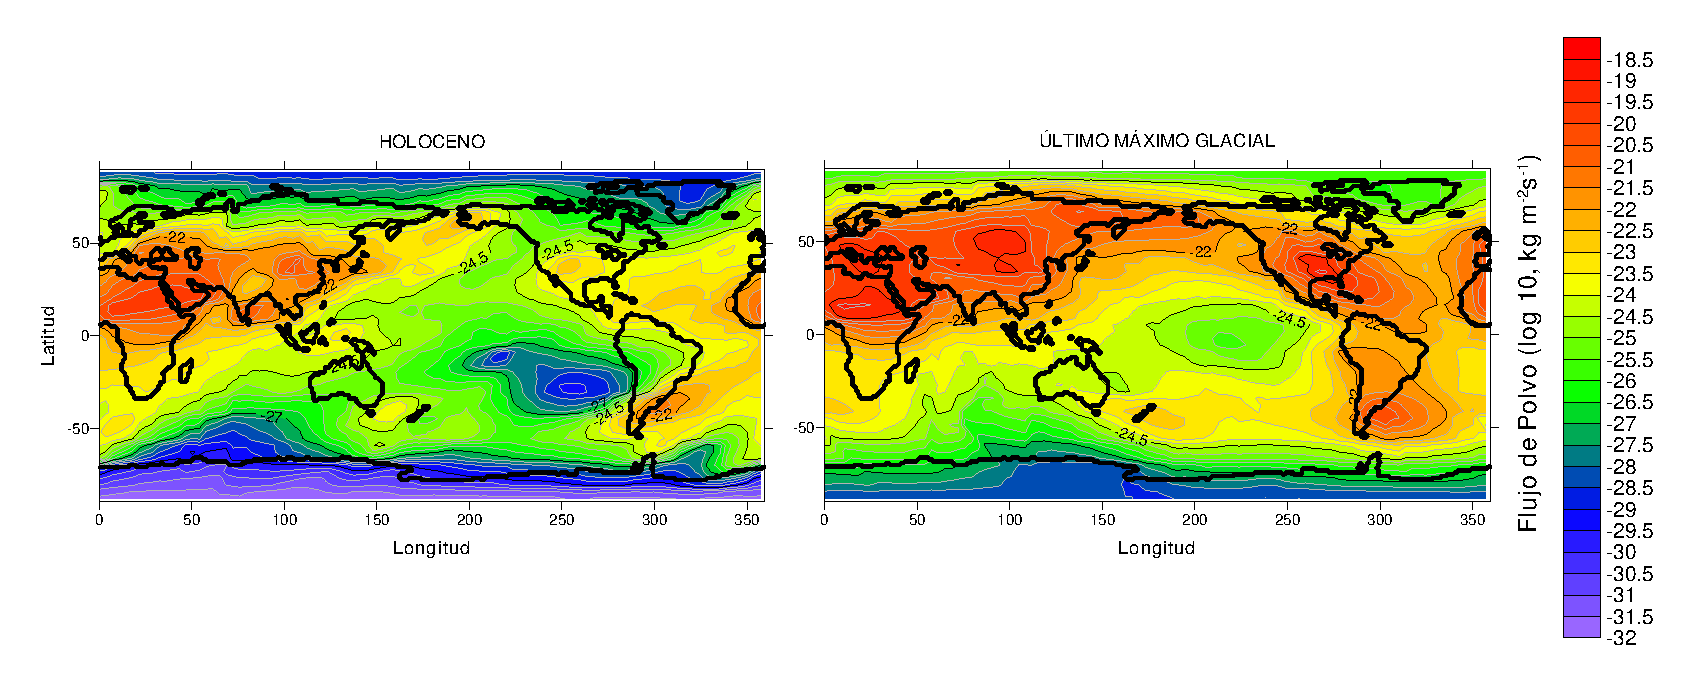
\includegraphics[width=1.1\textwidth]{Plot1_Lambert_2.pdf}
 \caption[Flujos de polvo \cite{lambert2015dust}]{Mapa global de flujos de polvo interpolados entre el periodo del Holoceno y el \'Ultimo M\'aximo Glacial. Datos obtenidos de \cite{lambert2015dust}.}
  \label{fig:Mapa_Lambert}\end{figure}

Los datos muestran que los flujos de depositaciones globales son distintos en los periodos presentados, dado que tanto para el Holoceno como UMG corresponden a 2278.559 Tg año$^{-1}$ y 7639.490 Tg año$^{-1}$ respectivamente. Entre las diferencias que se pueden apreciar entre ambos periodos, es que las fuentes de polvo se intensifican en el UMG en comparación al Holoceno. Así, durante el UMG las fuentes de América (norte y sur) son más pronunciadas y la mayor parte de la deposición en el océano Atlántico Norte parece provenir de América del Norte y de África del Norte por sobre Asia como se muestra durante el Holoceno. También durante este periodo en la zona de Groenlandia hay importante aportes provenientes de Siberia y Alaska, mientras que en la zona del giro subtropial del Pacífico Sur hay bajas concentraciones de depositación de polvo, sin embargo, aumenta hacia la parte sur lo que el autor asocia a productos de la interpolación que no están ratificados por mediciones. También se muestra un importante aporte de polvo que proviene de América del Sur, de las zonas desérticas hacia el océano Pacífico Sur y de la Patagonia hacia el Atlántico Sur. 

\subsection{Modelos PMIP}

La tercera fase de \textit{Palaeoclimate Modelling Intercomparison Project} (PMIP3) liberada el año 2012, es la primera versión PMIP en ser incluida en el \textit{Coupled Model Intercomparison Project} en su fase 5 (CMIP5) (actualmente se encuentra en su sexta fase), desarrollado por el Programa \textit{Word Climate Research} (WCRPs). El cual consta de un conjunto de modelos acoplados construidos con el propósito de evaluar la variabilidad climática, la relación y respuesta a distintos forzantes naturales. La fase quinta de CMIP esta dividida en dos categorías, experimentos a largo plazo y experimentos de periodos cercanos. No obstante, en ambos casos se realiza una simulación básica en la que se considera el periodo pre-industrial (1750) como simulación de control, en la que se evalúa la sensibilidad climática. En particular los modelos PMIP incluyen simulaciones que abarcan periodos extensos correspondientes al pasado, como el \'ultimo milenio (1000 a.p.), el Holoceno medio (6000 a.p.) y el \'Ultimo M\'aximo Glacial (21000 a.p.).

 {\bf MRI-CGCM3.} El modelo \textit{MRI-CGCM}3 perteneciente a PMIP3/CMIP5, desarrollado por el \textit{Instituto de Investigación Meteorológica de Jap\'on} (MRI por sus siglas en inglés) es una actualización de la versión PMIP2, \textit{MRI-CGCM2}. Es un modelo acoplado que consta de un modulo de interfase entre la superficie terrestre y la atmósfera (MRI-AGCM3), un modulo oceánico con cubierta de hielo (MRI.COM3) y un modulo de aerosol (MASINGAR mk-2). Todas las componentes están conectadas mediante ``Scup'' un flexible acoplado que permite hacer múltiples combinaciones.
 
 Los datos de polvo corresponden a la simulación MRI-CGCM3 de polvo en la que se utiliza el modelo \textit{Model of Aerosol Species in the Global Atmosphere} (MASINGAR mk-2). Cuya primera versión fue realizada y descrita por \cite{2003} Un modelo físico tridimensional que describe el transporte químico de aerosoles en la troposfera. Utilizado por la \textit{Japan Meteorological Agency} (JMA) para realizar pronósticos futuros de emisiones de polvo. Dentro de su parametrización no considera la estabilidad atmosférica, las variaciones de la velocidad de fricción límite y diferencias a partir de las propiedades del suelo, por lo que es considerado un modelo simple. No obstante, utiliza 4 especies de aerosoles entre ellos el sulfato de sal marina, carbonaceous, polvo mineral y aerosoles de sal marina \citep{2003}. Recibe los campos meteorológicos y las condiciones de superficie del \textit{Atmospheric General Circulation Model} (AGCM) el cual incluye características de la superficie terrestre mediante el \textit{Simple Biosphere} (SiB) \citep{yukimoto2012new}.  

 \begin{figure}[H]
\centering
  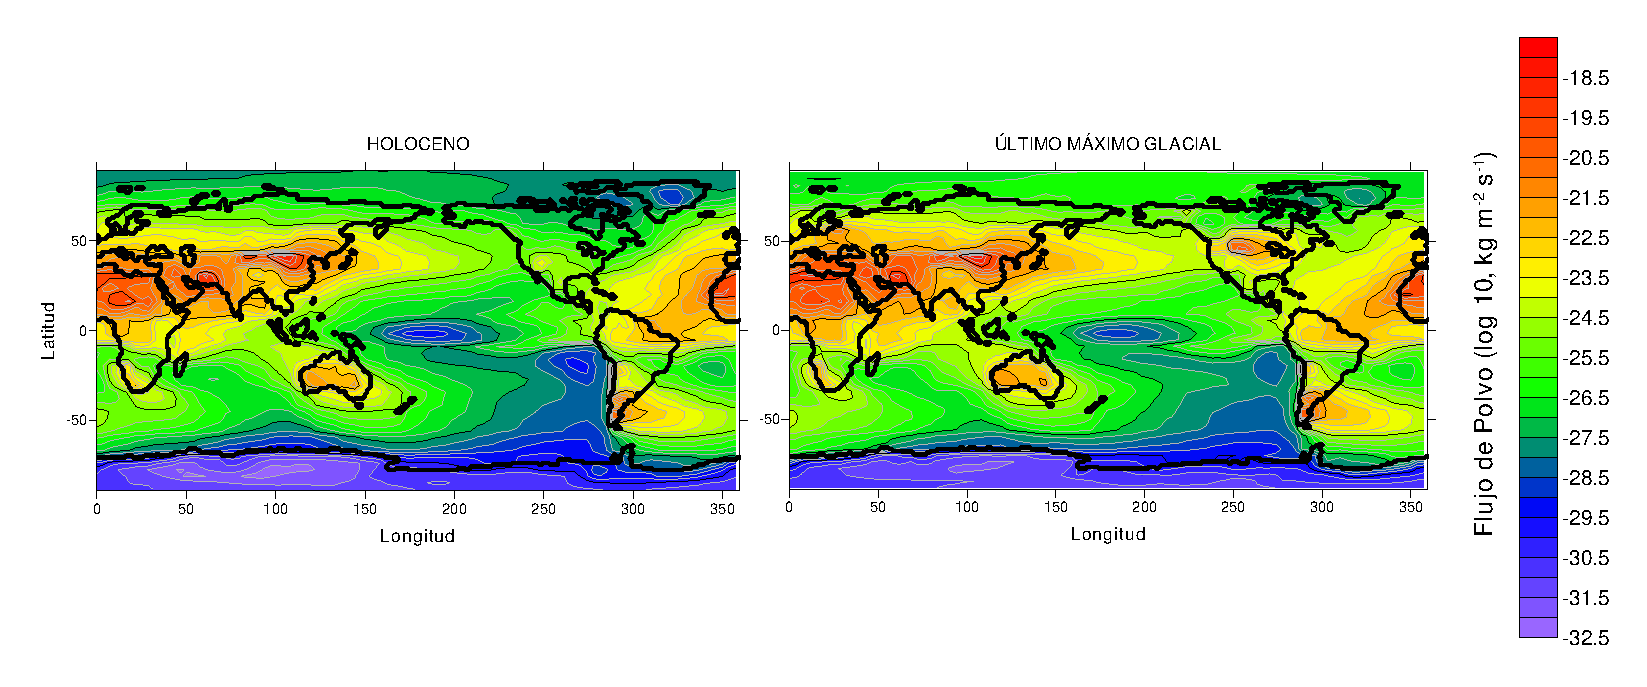
\includegraphics[width=1.1\textwidth]{Plot1_MRI.pdf}
  \caption[Flujos de polvo \cite{yukimoto2012new}]{Mapa global de flujos de polvo interpolados entre el periodo del Holoceno y el \'Ultimo M\'aximo Glacial. Datos obtenidos a partir \cite{yukimoto2012new}.}
  \label{fig:MRI}
\end{figure}

La depositación de polvo del modelo MRI-CGCM3, tanto en el Holoceno como en el UMG es de 2155.646  (Tg año$^{-1}$) para el Holoceno y 2965.467  (Tg año$^{-1}$) para el UMG. Donde las depositaciones de ambos periodos son similares, particularmente este efecto se aprecia en América del sur, donde durante el UMG no muestra flujo en la zona ecuatorial, mientras que en la zona patagónica existe un flujo que aporta en el Atlántico Sur, pero en general es similar al del Holoceno. 

 {\bf MIROC-ESM.} El modelo \textit{MIROC-ESM} perteneciente a PMIP3/CMIP5, fue desarrollado bajo el alero de los \textit{Earth system models} (ESMs) en la \textit{Japan Agency for Marine Earth Science and Technology} (JAMSTEC) en colaboración con el \textit{Center for Climate System Research} (CCSR), que estaban en búsqueda de un modelo que incluyera las retroalimentaciones del ciclo del carbono, es decir, que pudiera pronosticar las concentraciones de CO$_2$ atmosférico. Está basado en \textit{Model for Interdisciplinary Research on Climate} (MIROC3.2). MIROC-ESM es un modelo acoplado compuesto de un módulo de circulación atmosférica (MIROC-AGCM 2010), un módulo de circulación oceánica con una componente de hielo (COCO 3.4), un modelo de superficie de la tierra (MATSIRO), un módulo de aerosoles (SPRINTARS 5.00), y un componente de ecosistemas marinos (nutrientes, especies de plancton, NPZD) y terrestres (dinámica vegetacional, SEIB-DGVM), también se introduce una componente nueva relacionado con la química atmosférica (CHASER 4.1). Todos los módulos están conectadas mediante ``K-1'' un acoplador de flujo. 

Los datos de polvo presentados corresponden a la simulación de polvo MIROC-ESM en la que se utiliza el modelo \textit{Spectral Radiation-Transport Model for Aerosol Species} (SPRINTARS). El cual es un modelo físico tridimensional que predice la mezcla de los principales aerosoles troposféricos entre ellos: sulfato, polvo del suelo, carbonaceos (carbono orgánico (OC) y carbón (BC)), sal de mar, y precursores de gases de sulfato (dióxido de azufre (SO$_2$) y sulfuro de dimetilo (DMS)). Entre los procesos de transporte de estos gases está considerado la emisión, advección, difusión, química del azufre, deposición humeda, deposición seca y depositación gravitacional. El módulo es impulsado por un modelo de circulación atmosférica del CCSR que involucra procesos radiativos \citep{takemura2000global,sueyoshi2013set}.  

 \begin{figure}[H]
\centering
  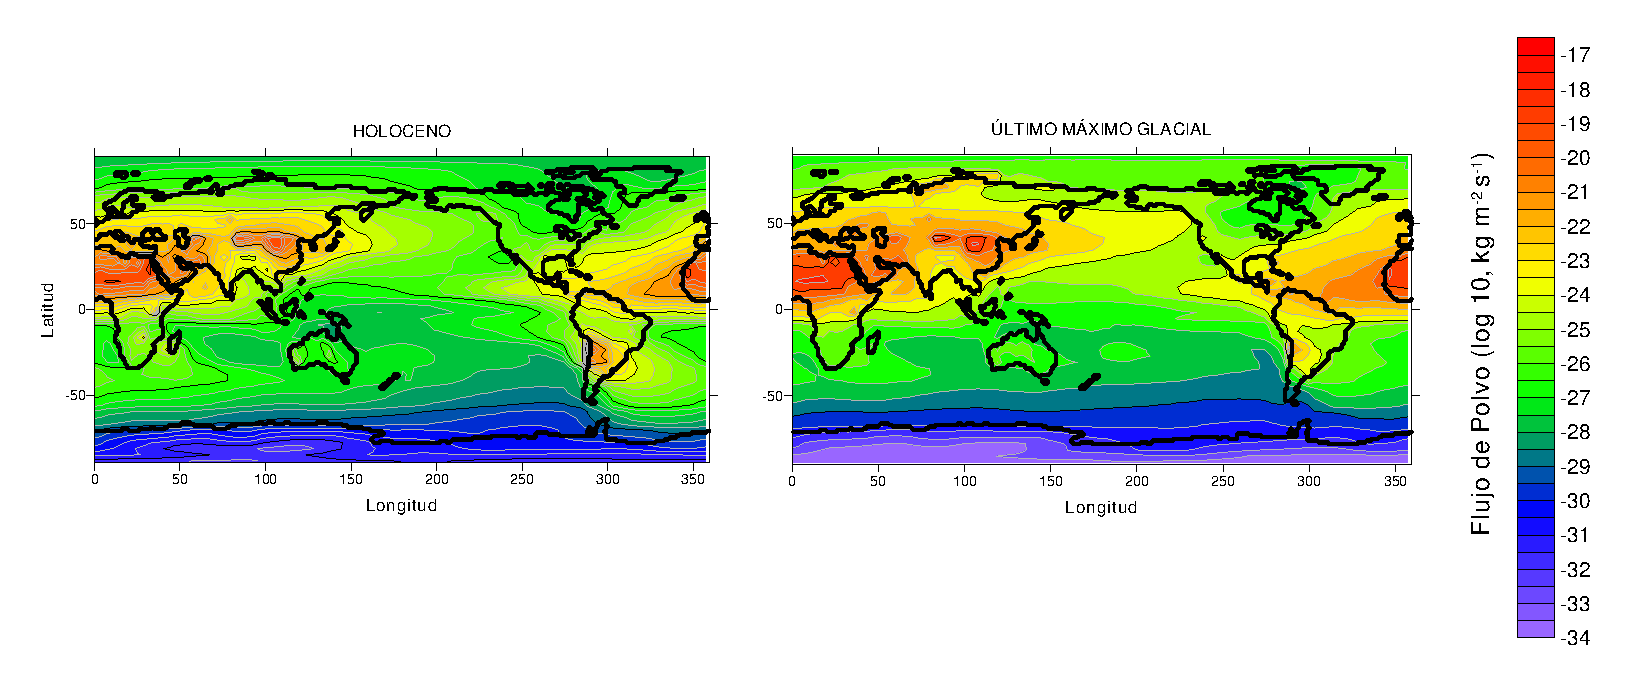
\includegraphics[width=1.1\textwidth]{Plot1_MIROC.pdf}
  \caption[Flujos de polvo \cite{sueyoshi2013set}]{Mapa global de flujos de polvo interpolados entre el periodo del Holoceno y el \'Ultimo M\'aximo Glacial. Datos obtenidos de \cite{sueyoshi2013set}.}
  \label{fig:MIROC}
\end{figure}

La depositación de polvo global simuladas por MIROC-ESM para el Holoceno y UMG, son de 2351.565 Tg año$^{-1}$ y 6674.501 Tg año$^{-1}$ respectivamente. 

Entre las bases de datos se puede apreciar un aumento de los flujos de polvo, habiendo una mayor producción durante el UMG que durante el Holoceno. No obstante, el modelo no presenta grandes fuentes de polvo en el Hemisferio Sur, lo que se refleja particularmente en la zona patagónica de Sur América, la cual es sabido es una importante fuente de polvo glaciogénico para los Océanos del Sur, de igual manera en la zona de Australia/Nueva Zelandia tampoco se aprecia una fuente de polvo. En las zona del Pacífico Ecuatorial si bien existe una lengua de polvo, es un aporte muy reducido.   

{\bf Takemura.} La distribuci\'on global de polvo presentado a continuaci\'on fue desarrollado a partir del modelo clim\'atico de aerosol SPRINTARS, junto con la inclusi\'on de la interacci\'on entre los cristales de hielo y las part\'iculas de aerosol. relacionados con la emisión de flujos de polvo aerosoles (velocidad del viento cercano a la superficie, de la cubierta vegetacional, y del índice folear, humedad del suelo y cantidad de nieve), así también las características relacionadas con el flujo de emisión de sal marina y la parametrización relacionada con la interacción entre los aerosoles y cristales de hielo. Para más detalle revisar el articulo de \cite{takemura2009simulation}.

\begin{figure}[H]
\centering
  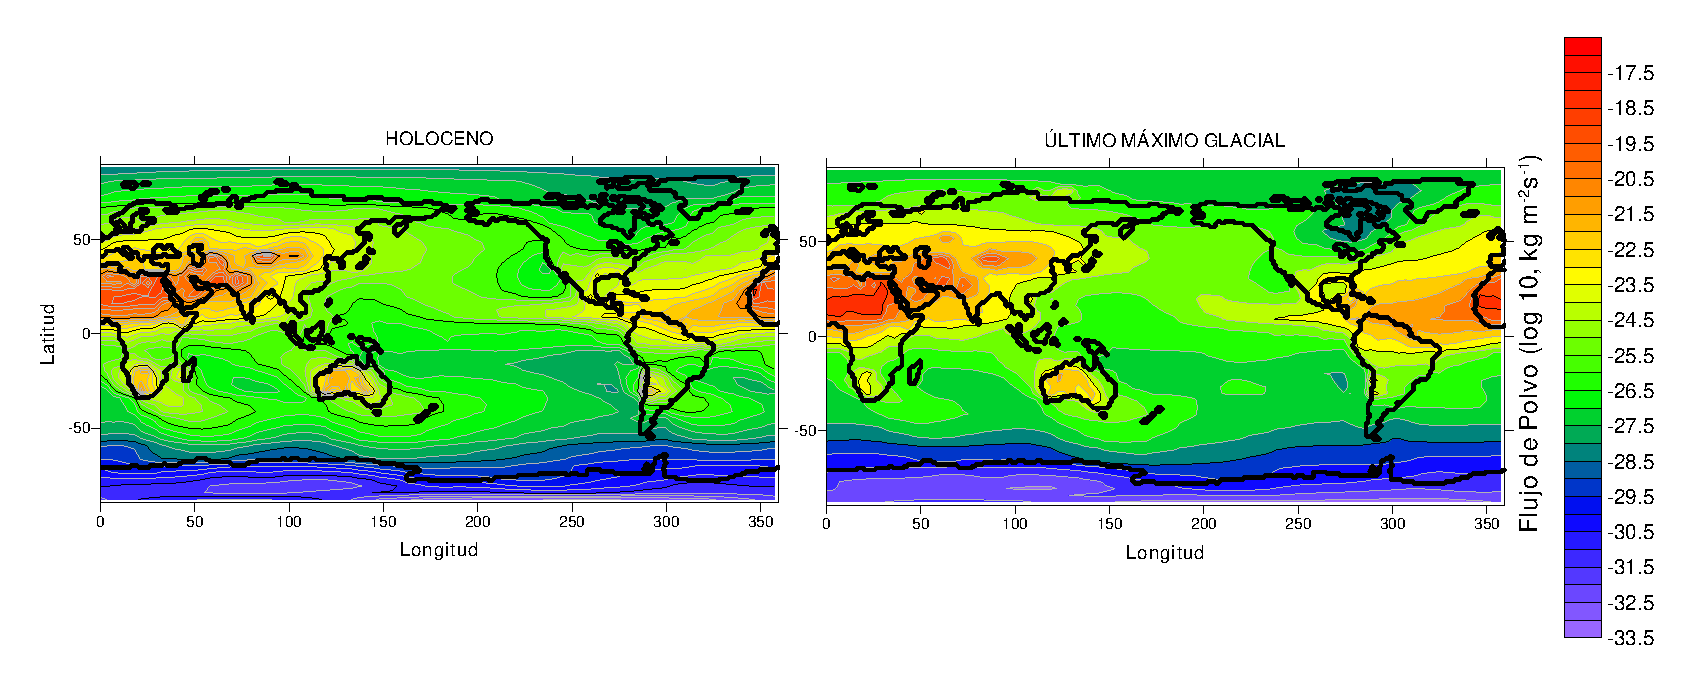
\includegraphics[width=1.1\textwidth]{Plot1_Takemura.pdf}
  \caption[Flujos de polvo \cite{takemura2009simulation}]{Mapa global de flujos de polvo interpolados entre el periodo del Holoceno y el \'Ultimo M\'aximo Glacial. Datos obtenidos de \cite{takemura2009simulation}.}
  \label{fig:Takemura}
\end{figure}

Los flujos de depositación globales de polvo a partir de esta simulación tienen valores de 2535.295 Tg año$^{-1}$ para el periodo del Holoceno y 5756.909 Tg año$^{-1}$ durante el UMG. Según \cite{takemura2009simulation} los flujos obtenidos se corresponden de buena manera con los datos de testigos de testigos de hielo y sedimentos marinos. Si bien durante el UMG la simulación mostró una expanción de las fuentes del Sahara hacia el sur y hacia el Norte sobre Europa del Este y Asia Central, hay una predominancia de altas tasas de deposición en latitudes altas del Hemisferio Norte mientras que en el Hemisferio Sur en zonas como la Antártica se aprecia una casi nula deposición (siendo que los datos muestran que hay una fuente primaria en la Patagonia), así mismo tanto Australia como África Austral muestran bajas tasas de depositación. 

{\bf Albani.} Para la construcción del campo de polvo ``\textit{Albani}'', se utilizó el modelo acoplado \textit{Community Earth System Model Version 1} (CESM1). El cual es un modelo de sistema tierra global incluido dentro de CMIP5, que está compuesto por cuatro módulos separados que representan la componente atmosférica, oceánica, de superficie terrestre y cubierta de hielo marina. Donde \citep{albani2014improved} hizo uso de la componente atmosférica, la \textit{Community Atmosphere Model version 4} (CAM4) y su versión posterior la \textit{Community Atmosphere Model version 5} (CAM5) (www.cesm.ucar.edu) ajustando para ello un conjunto de parametrizaciones físicas relacionadas con el polvo (erosibilidad del suelo, tamaño de distribución de polvo emitido, deposición húmeda y propiedades ópticas). Para la simulación de polvo del UMG se utilizó el subconjunto \textit{ Community Climate System Model} (CCSM4). Los resultados de las simulaciones son comparados con datos observacionales utilizando para ello el \textit{Aerosol optical depth} (AOD) en su versión 2, que da una estimación de la cantidad de haces de luz que se impide que lleguen a la superficie producto de la presencia de particulas de aerosoles en la columna de aire (como el polvo, la bruma, etc). Para la superficie se utilizó la concentración atmosférica y el flujo de deposición de polvo tomados de la \textit{University of Miami Ocean Aerosols Network}, también se utilizaron datos de estaciones, aunque estos últimos no fueron utilizados en la optimización de los modelos. 

\begin{figure}[H]
\centering
  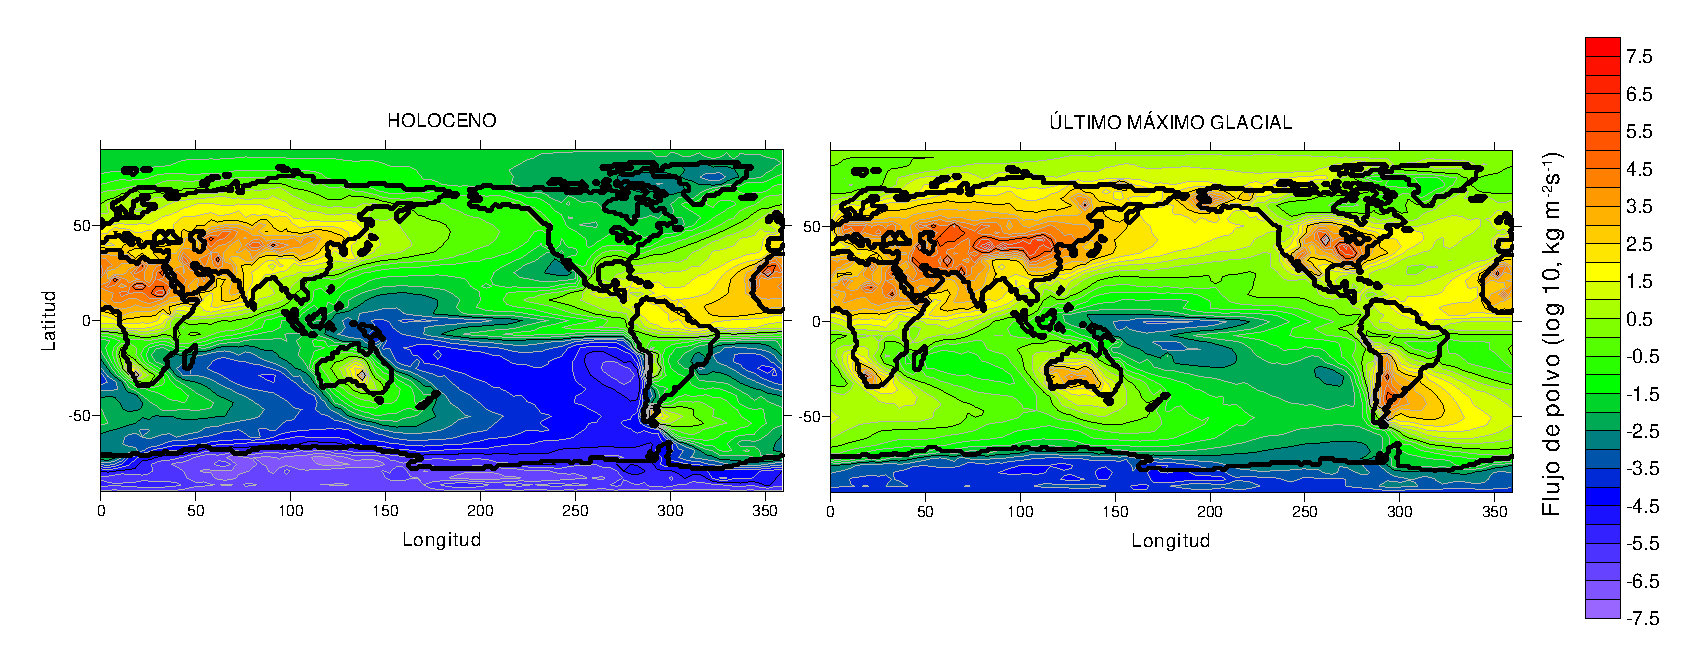
\includegraphics[width=1.1\textwidth]{Plot1_Albani.pdf}
  \caption[Flujos de polvo \cite{albani2014improved}]{Flujos de campos de polvo desarrollados mediante el modelo acoplado \textit{Community Earth System Model Version 1} (CESM1).  A la derecha el periodo del Último Máximo Glacial y a la izquierda el Holoceno. Datos obtenidos de \cite{albani2014improved}.}
  \label{fig:Albani}
\end{figure}

Los modelos tienden a mostrar altas emisiones con altas cargas, y periodos de vida más cortos durante el Holoceno en comparación a los datos de observaciones. Mientras que durante el UMG las magnitudes estimadas por el modelo son representativas de observaciones en paleo-datos en los 4 ordenes de magnitud abarcados por los datos. Donde alcanzan 2.2 veces lo calculado por unos de los modelos de 
\textit{Community Earth System Model Version 1} (CESM1), abarcando valores de $6289$ Tg/a. Además que el 20\% de las emisiones provienen de fuentes glaciogénicas, con una vida media de 2.2 días y una carga de polvo es 37.4 tg/año \citep{albani2014improved}. 


\subsection*{Análisis de datos}

Entre los campos de flujos de polvo las simulaciones realizadas por \cite{takemura2009simulation} (basada en el modelo \textit{MIROC-ESM}), reflejan una carencia de fuentes de polvo en el Hemisferio sur durante el UMG lo que se condice con el modelo \textit{MIROC-ESM}. No obstante, tanto \textit{MRI-CGCM3} como la reconstrucción \textit{Lambert} muestran un aumento en el aporte a esta zona en el UMG, mayormente en el Atlántico Sur, lo que los flujos de \textit{Albani} intensifican presumiblemente sobrestimando las concentraciones reales, pero mostrando la vital importancia de las fuentes glaciogenicas durante estos periodos. Por otro lado, todas las simulaciones y reconstrucción exponen una considerable intensificación de las fuentes de polvo en el Hemisferio Norte en el UMG, siendo \textit{Lambert} uno de los que más diferencias muestran en esta zona (ver imagen \ref{fig:Amp}). Además respecto de la zona del Pacífico Ecuatorial, tanto \textit{MIROC-ESM} y \textit{Takemura} revelan altas depositaciones durante el UMG, sin embargo, es en la zona este de la región donde se aprecia una lengua de depositación de polvo que es compartida por todos los modelos. 

\section{Pre-procesamiento}

\begin{figure}[H]
\centering
  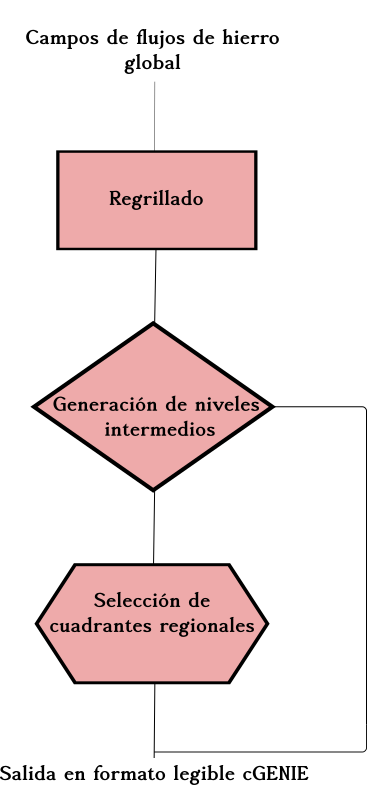
\includegraphics[width=0.29\textwidth]{diagrama_met1.png}
  \caption[Pre-procesamiento de datos]{Estructura del pre-procesamiento de los flujos de campo de polvo.}
  \label{fig:diagrama_met1}
\end{figure}

En esta etapa se realizan tres procesos diferentes que serán posteriormente utilizados como input en el modelo cGENIE: 1) la redimención de campos de polvo globales de los periodos del Holoceno y LGM, 2) la generación de niveles intermedios equidistantes entre los periodos anteriores y 3) la generación de campos regionales desde el campo intermedio posterior al Holoceno hasta el UMG. 

\begin{description}
  \item[1) Regrillado de campos de polvo globales Holoceno y UMG:]

Los 5 campos de polvo expuestos en la sección 4.1 para el Holoceno y para el UMG, tienen una grilla que es de 128x64 celdas en cuatro casos (Lambert, Takemura, MIROC-ESM, MRI-CGCM3) y una de 192x268 celdas (Albani). Para el modelo cGENIE es necesario traspasar todos los campos a una grilla cuadrada de 36x36, que serán los nuevos campos de flujos de polvo globales tanto para el Holoceno (5 campos) y para el UMG (5 campos). 

  \item[2) Campos de polvo intermedios globales Holoceno y UMG:]

Con el propósito de observar los cambios en la concentración de CO$_2$ atmosférico que se dan entre el periodo del Holoceno hasta el UMG, y sobre la base de los diferentes inputs de campos de polvo previamente regrillados (\textit{item 1}), se realiza una interpolación x-espaciada, creando con ello 8 diferentes escenarios intermedios de polvo. Éstos en conjunto con el \textit{item 1} generan 10 niveles que van desde el Holoceno hasta el UMG incluyendo ambos periodos.

   \item[3) Campos de polvo intermedios regionales:]

Para ver el efecto que cada zona HNLC (ver figura \ref{fig:Grilla4}) aporta en la captura de pCO$_2$ producto de la fertilización con hierro, se procedió a generar nuevos campos de polvo a partir de los 10 producidos de la combinación del \textit{item 1 e item 2}. 

Para ello, en primera instancia la concentración de polvo correspondiente al Holoceno (nivel 1) se inserta en cada punto de grilla que no tenga asociada una zona HNLC de interés (dejando su concentración original), este proceso se reproduce en todos los niveles de polvo de la misma forma (hasta el niveles 10). Ésto produce 10 campos de polvo donde la única variación de polvo a lo largo del tiempo (que abarca el Holoceno y UMG) se da en la zona HNLC seleccionada (manteniendo sus datos originales en todos los niveles). Este proceso se replica para cada zona HNLC, generando finalmente 10 campos de polvo por región, es decir, 40 campos de polvo por casa caso (Albani, Lambert, MIROC-ESM, MRI-CGCM3, Takemura). 
\end{description}

\subsection{Pre-procesamiento modelo cGENIE}

Una vez generados los flujos de campos de polvo globales desde el Holoceno hasta el UMG y los flujos de polvo intermedios, se procede a subir los archivos en la configuración de cGENIE ejecutado en un cluster de la Universidad de BRISTOL.

\begin{figure}[H]
\centering
  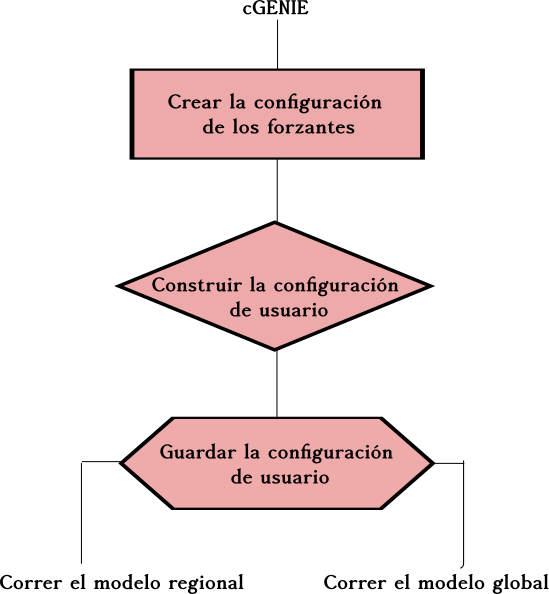
\includegraphics[width=0.5\textwidth]{diagrama_met2.png}
  \caption[Pre-procesamiento modelo cGENIE]{Estructura del pre-procesamiento de los flujos de campo en cGENIE.}
  \label{fig:diagrama_met2}
\end{figure}

 Para configurar un experimento en el modelo cGENIE, es necesario ingresar en el directorio localizado en cgenie.muffin/genie-forcings, dado que aqu\'i es donde son almacenado los forzantes y contiene todos los archivos que definen las propiedades geoqu\'imicas que modificaran la informaci\'on acerca de como un forzante cambiar\'a en el tiempo. En este caso el trazador corresponde a los campos de flujos de polvo generados en el \textit{item 1/item f2 e item3} de la secci\'on 4.2. Se especifican los cambios en las concentraciones del forzante en el tiempo ``Condiciones de contorno del modelo''. 

 Así, en este caso se crearon manualmente dos carpetas en genie-forcings, una con el nombre ``worjh2.FeMODELO\_All.level*'' y otra llamada ``worjh2.FeMODELO\_Regi\'on.level*'', para simulaciones globales y regionales respectivamente. Esto se replic\'o para todos los niveles de polvo en cada caso. 

Dentro de cada una de estas carpetas se incorporaron 5 archivos: 

\begin{itemize}
  \item[1) ] \textbf{biogem\_force\_flux\_sed\_det\_SUR.dat} ``biogem\_force\_*\_I.dat''. Especifica la ubicación en el océano del forzante geoquímico que será aplicado (componente espacial). En este caso la grilla de flujo de polvo es de dos dimensiones (grupos de datos que contienen filas (j) y columnas (i)), en unidades de mol a$^-1$. 
  \item[2) ] ``configure\_forcings\_atm.dat''. Definición de forzantes atmosféricos interactuando en el modelo. Para esta simulación no se definen. 
  \item[3) ] ``configure\_forcings\_ocn.dat''.Definición de forzantes oceánicos interactuando en el modelo. En esta simulación no se definen. 
  \item[4) ] ``\textbf{configure\_forcings\_sed.dat}''. Definición de forzantes sedimentarios interactuando en el modelo. Para esta simulación se definen forzantes provenientes de sedimentos terrestres (polvo). 
  \item[5) ] biogem\_force\_flux\_sed\_det\_sig.dat ``biogem\_force\_*\_II.dat''. Define la componente temporal del forzante (variación en el tiempo). 
Se construye a partir de la magnitud del forzante que es aplicado en la posición $(i,j)$ en un tiempo $_{(t)}$, m\'as un modificador S$_{(t)}$ que es dependiente del tiempo, por la diferencia entre los dos campos \textit{item 5 - item 1}, es decir: 
 \begin{equation} \label{eq:met1}
F_{(i,j),(t)}= biogem\_force\_*\_I_{(i,j)}\ +\ S_{(t)}\ \times\ (biogem\_force\_*\_II_{(i,j)}\ -\ biogem\_force\_*\_I_{(i,j)})
\end{equation}
El valor del trazador de escala ($S_{(t)}$) es interpolado desde los contenidos de la se\~nal forzante del archivo 
biogem\_force\_flux\_sed\_det\_SUR.dat.
\end{itemize}

Luego de crear las carpetas y archivos para todos los niveles de polvo y para cada tipo (regional o global), es que se crearon los archivos y carpetas de configuraci\'on (ver figura Anexo \ref{tabla:U-conf}). Este proceso se realiza en el directorio \textit{genie-Userconfig} dentro del directorio \textit{cgenie.muffin}. \newpage

\section{Experimento, modelo cGENIE}

 \begin{figure}[H]
\centering
  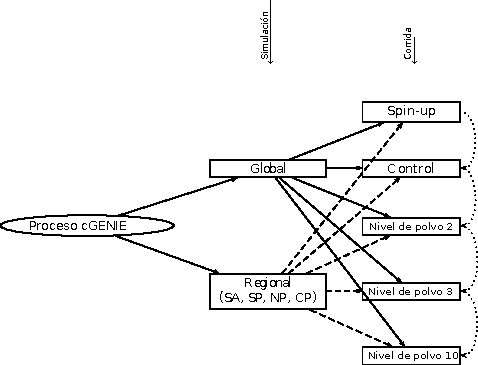
\includegraphics[width=0.7\textwidth]{runcGENIEpdf.pdf}
  \caption[Estructura de la Simulación en cGENIE]{Estructura de la Simulación en cGENIE. Se aprecia el Spin-up (configuración básica) para posteriormente representar la evaluación progresiva de los flujos de polvo.}
  \label{fig:run}
\end{figure}

La simulación fue desarrollada en tres etapas: 1) se realiz\'o una configuración básica necesaria para dar una consistente iniciación al modelo cGENIE (spin-up), 2) se ejecut\'o una simulación de control para verificar que el modelo ratifique los valores observados y 3) se evaluaron los niveles de campos de polvo desde el Holoceno hasta el UMG en todos los casos dados (globales y regionales). 

\subsection*{Configuración general}

Todos las simulaciones que se expondrán a continuación (spin-up, control, experimentos), fueron corridos por un intervalo de tiempo de 10000 años (para la estabilización, figura \ref{fig:Control}). En este caso, dado que buscamos evaluar el efecto del hierro en la bomba biológica y cómo esto afecta la concentración de CO$_2$, la componente de biogeoquímica oceánica correspondiente al módulo BIOGEM toma una importante relevancia. Mientras que la configuración básica seleccionada es \textit{cgenie.eb\_go\_gs\_ac\_bg.worjh2.BASEFe}, la cual representa los módulos presentes en la tabla \ref{tabla:Met1}, la configuración continental, la resolución y trazadores escogidos incluyendo el ciclo del hierro marino. 

\begin{description}
\item[1) Spin-up:] Con el propósito de establecer las parametrizaciones del modelo cGENIE en las condiciones climatológicas del periodo preindustrial es que se desarrolla un spin-up. Para lo cual, se utilizó el flujo de polvo del Holoceno de cada modelo/reconstrucción de polvo. En esta etapa se fija el CO$_2$ en 278 ppm (concentración periodo preindustrial), con un ``biogem\_force\_*\_II.dat'' fijado en cero lo que significa que no tomará los valores del forzante de polvo que le estamos ingresando (ver figura \ref{fig:SPIN-UP}). 

De aquí en adelante todos los experimentos fueron corridos dependiendo del final del estado del spin-up. 

\item[2) Control:] Se desarroll\'o una simulación de control aplicando los mismo campos de polvo usados por el Spin-up (Holoceno), pero sin fijar la concentración atmosférica de CO$_2$. La figura \ref{fig:Control} de las simulaciones de control, muestra una estabilización alrededor de los 2000 años para todos los modelos y reconstrucciones.

\item[3) Experimentos:] Finalmente procedemos a correr el modelo desarrollando tantos las evaluaciones del efecto del hierro en la captura de CO$_2$ a nivel global como regional (zonas HNLC).
En la l\'inea de comando del cluster BRISTOL, dentro del directorio genie-main ingresamos el comando: ( \$ qsub -j y -o cgenie\_log -V -S /bin/bash runmuffin.sh ) junto con una lista de parámetros que permiten correr el modelo.\\
\$... ./runmuffin \#1 \#2 \#3 \#4 (\#5)

Estos par\'ametros son:\\
\#1 el nombre de la configuraci\'on b\'asica requerida para el modelo, en este caso ser\'a\\
\textit{cgenie.eb\_go\_gs\_ac\_bg.worjh2.BASEFe}.\\
\#2 nombre del subdirectorio que contiene los archivos ``user-config'', en nuestro caso ``DUST''. \\
\#3 nombre del archivo de configuraci\'on (user-config).\\
\#4 longitud de la corrida en a\~nos, en nuestro caso 10000 a\~nos. Para el caso del \textit{spin-up} s\'olo se ocupan los par\'ametros definidos hasta aqu\'i.  \\ 
\#5 corrida de arranque (periodo preindustrial), en nuestro caso ``worjh2.PO4Fe.SPIN''. Necesario para la simulaci\'on de control y experimento con polvo. 

Al finalizar la corrida los archivos de salida (resultados) son almacenados dentro del directorio \textit{cgenie\_output}. 
\end{description}

\begin{figure}[H]
\centering
 \includegraphics[width=1.2\textwidth]{../../Figuras/Series/Series_Holoceno.png}
 \caption[Series de pCO$_2$ de simulación de control]{Serie de tiempo de pCO$_2$ obtenidos a partir de las simulaciones de control realizadas mediante el modelo cGENIE, para el periodo del Holoceno de todos los campos de polvo.}
  \label{fig:Control}
\end{figure}

\section{Post-procesamiento}

Los archivos de $pCO_2$ obtenidos del modelo cGENIE, son procesados en el software \textit{Matlab} en el cual se procede de la siguiente manera: 

\begin{itemize}
    \item[a) ] Se seleccionaron los últimos 10 datos del archivo biogem\_series\_atm\_pCO2.res ubicado en cgenie\_output/user\_config/biogem, correspondientes a niveles de pCO$_2$ de la parte estable de la simulación. 
    \item[b) ] Sacamos la diferencia de pCO$_2$ entre cada nivel desde el periodo preindustrial (nivel 1) hasta el \'Ultimo M\'aximo Glacial (nivel 10).
    \item[c) ] En el caso del flujo global, se hiz\'o una mediana del pCO$_2$ obtenido con cGENIE, para los 10 periodos (niveles).
    \item[d) ] Posteriormente se graficaron las diferencias de $pCO_2$ respecto del hierro en cada nivel y se ajust\'o una curva a los datos.
    \item[e) ] Por otro lado, se calculó en porcentaje la reducción de cada nivel para cada zona
de interés respecto del UMG. De esta manera, se obtuvo un porcentaje relativo del aporte de cada zona HNLC a la reducción total de CO$_2$ (ver Anexos) para cada modelo y recontrucción ingresada en cGENIE.
\end{itemize}





\chapter{Resultados}

% !TEX root = ../Tesis_NataliaOpazo.tex 

A continuación se presentan los efectos generados por la inserción de los campos de flujo de polvo en los niveles de pCO$_2$ atmosférico según el modelo cGENIE, entre el periodo del Holoceno hasta el UMG. 

\section{Resultados globales}

En la figura \ref{fig:All}, la trayectoria del nivel de pCO$_2$ en todas las simulaciones pueden ser explicada por una función logaritmo. Sin embargo, Takemura muestra una pequeña desviación en el nivel 7 (con aproximadamente 9.5 ppm de reducción). Sin embargo, lo anterior no se condice con el aumento progresivo de polvo desde el Holoceno hasta el UMG para este caso. 

La simulación Albani es la que muestra mayor reducción de pCO$_2$ ($\sim 21$ ppm.). Seguido por el modelo MIROC-ESM ($\sim 20$ ppm). La máxima captación de Albani, puede ser producto de la diferencia intermedia de polvo entre el periodo del Holoceno y del UMG en comparación a los otros casos. Albani además, posee los niveles más altos de depositación de polvo durante el periodo del Holoceno (aunque es el tercer flujo de polvo durante el UMG). Esto habría dado un importante input inicial al modelo cGENIE que se mantuvo con valores altos hacia el final de la simulación (UMG). \newpage

\begin{figure}[H]
        \begin{subfigure}[b]{0.5\textwidth}
                \includegraphics[width=\linewidth]{../../Figuras/Globales/Albani/All}
                \caption{Albani}
                \label{fig:A_All}
        \end{subfigure}%
                \begin{subfigure}[b]{0.5\textwidth}
                \includegraphics[width=\linewidth]{../../Figuras/Globales/Lambert/All}
                \caption{Lambert}
                \label{fig:L_All}
        \end{subfigure}%

        \begin{subfigure}[b]{0.5\textwidth}
                \includegraphics[width=\linewidth]{../../Figuras/Globales/Takemura/All}
                \caption{Takemura}
                \label{fig:T-All}
        \end{subfigure}%
        \begin{subfigure}[b]{0.5\textwidth}
                \includegraphics[width=\linewidth]{../../Figuras/Globales/MIROC-ESM/All}
                \caption{MIROC-ESM}
                \label{fig:MI-All}
        \end{subfigure}
        
        \begin{subfigure}[b]{0.5\textwidth}
                \includegraphics[width=\linewidth]{../../Figuras/Globales/MRI-CGCM3/All}
                \caption{MRI-CGCM3}
                \label{fig:MR-All}
        \end{subfigure}
        \caption[Series de reducci\'on de $pCO_2$ de flujos globales de polvo]{Series de reducci\'on de $pCO_2$ obtenidos mediante simulaci\'on cGENIE, desde el Holoceno hasta el \'Ultimo M\'aximo Glacial para flujos de polvo globales.}\label{fig:All}
\end{figure}

 La simulación Lambert es la que presenta mayor diferencia entre el nivel de polvo del Holoceno y el UMG. Este tiene lo más elevados flujos de polvo para el UMG, dando una reducción de $\sim 16.5$ ppm. La simulación Lambert tiene el tercer valor más alto de disminución de pCO$_2$ atmosférico, seguido por el modelo Takemura ($\sim 16$ ppm.). Este último tiene los mayores flujos de polvo en el Holoceno pero capturas más bajas que Lambert hacia el UMG. La simulación MRI-CGCM3 posee los menores flujos de polvo y presenta la menor disminución de pCO$_2$, estimada en aproximadamente 9 ppm. \newpage

\section{Resultados regionales}
A continuaci\'on se presentan los resultados correspondiente a cada zona HNLC que se muestra en la figura \ref{fig:Grilla4}.

\subsection{Pac\'ifico Norte}

\begin{figure}[H]
\centering
 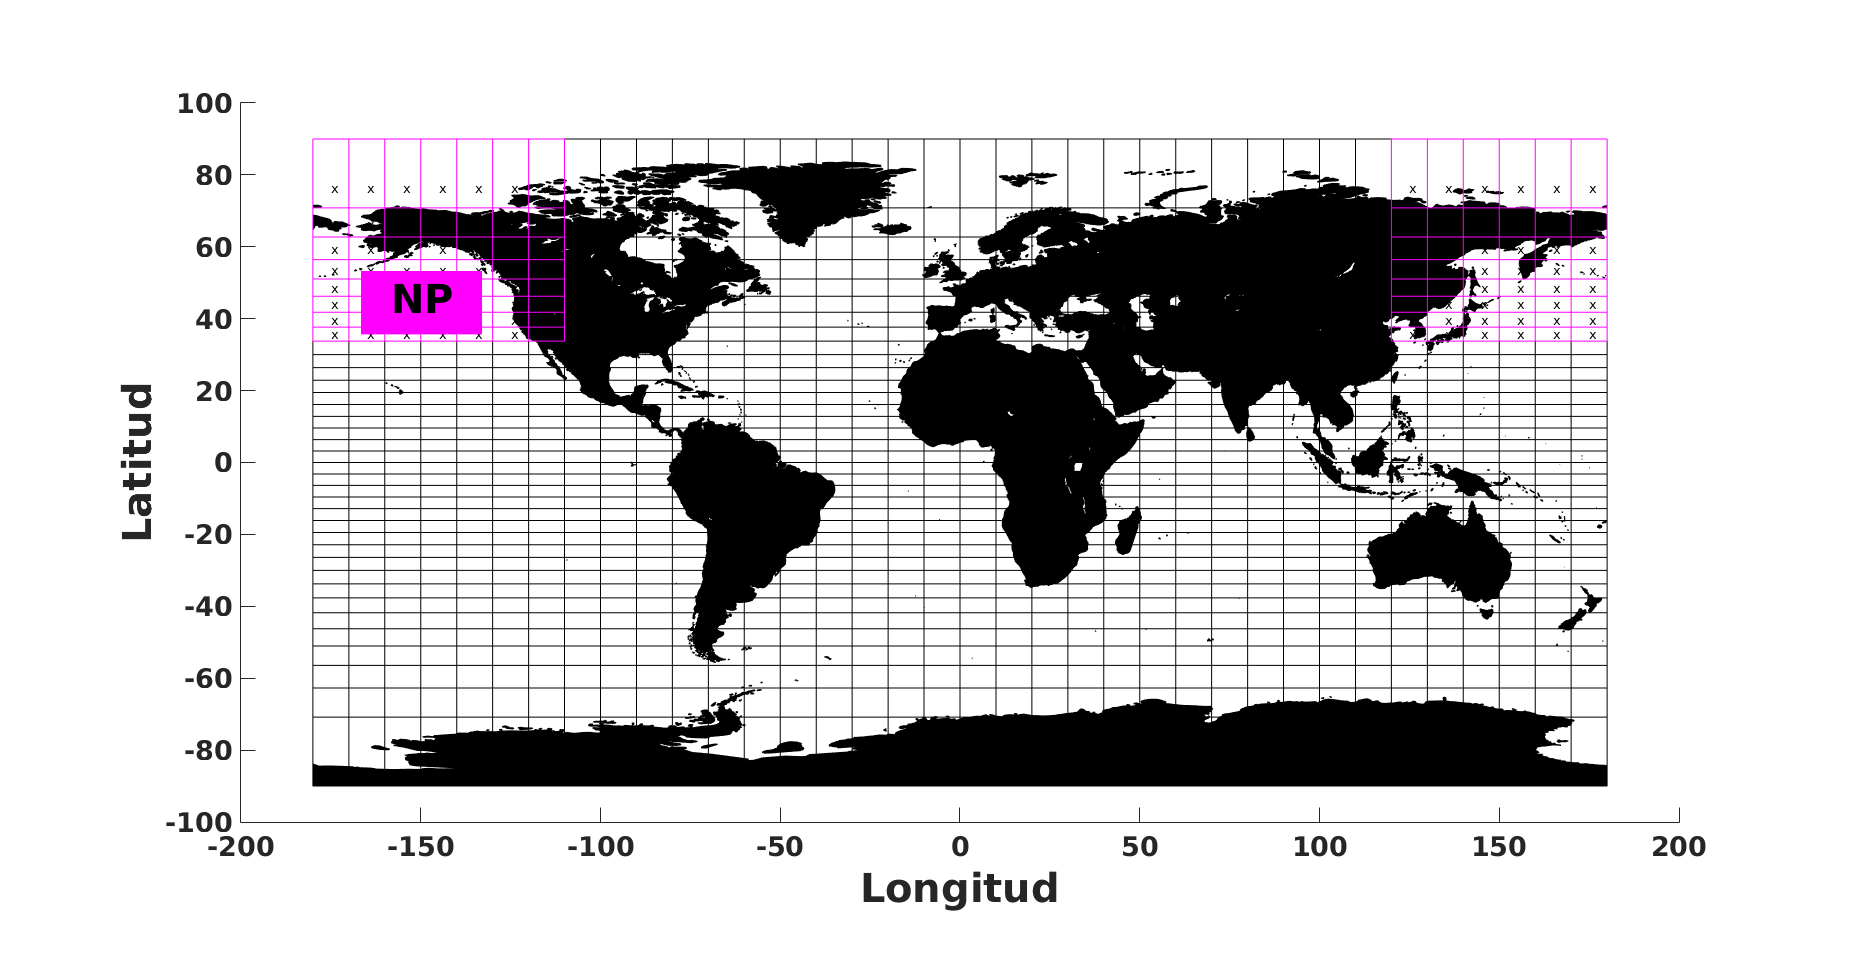
\includegraphics[width=0.8\textwidth]{mapa3_2_NP.png}
 \caption[Figura región del Pacífico Norte]{Mapa global, que muestra la región del Pacífico Norte que fue aislada en la simulación cGENIE.}
  \label{fig:Mapa_NP}
\end{figure}

\begin{table}[H]
\centering
\begin{tabular}{|c|c|c|c|c|}
\hline
& \multicolumn{4}{c|}{Reducci\'on de $pCO_2$ global} \\
\cline{2-5}
Modelo& Ajuste & Par\'ametros & R-cuadrado ($R^2$) & RMSE\\
\hline \hline
Lambert  & Logar\'itmico  & p1=-29.66, p2=5805 y p3=3.495 & 0.9975 & 0.0945 \\ \hline
Albani & Logar\'itmico & p1=-18.23, p2=-2382 y p3=-2382 & 0.9995 & 0.0613\\ \hline
Takemura & Logar\'itmico & p1=-16.09, p2=291 y p3=2.524 & 0.9999 & 0.0034\\ \hline
MIROC-ESM & Logar\'itmico & p1=-50.18, p2=3916 y p3=6.65 & 0.9984 & 0.0863
\\ \hline
MRI-CGCM3 & Logar\'itmico & p1=-39.01, p2=-126.5 y p3=5.074 & 0.9998 & 0.0132\\ \hline
\end{tabular}
\caption[Coeficientes del ajuste NP]{Caracter\'isticas de los ajustes realizados a las reducciones globales de $pCO_2$, a partir de los resultados del modelo cGENIE. El ajuste general es logar\'itmico, 
su ecuaci\'on est\'andar es: $ f(x)=p1 + \frac{p2}{x} + p3*log(x)$. Donde f(x) es la reducci\'on de $pCO_2$ y x, el flujo de polvo de cada nivel para la zona del Pacífico Norte. } 
\label{tabla:NP}
\end{table} \newpage

 \begin{figure}[H]
        \begin{subfigure}[b]{0.5\textwidth}
                \includegraphics[width=\linewidth]{../../Figuras/Regionales/Albani/NP}
                \caption{Albani}
                \label{fig:A_R_NP}
        \end{subfigure}%
                \begin{subfigure}[b]{0.5\textwidth}
                \includegraphics[width=\linewidth]{../../Figuras/Regionales/Lambert/NP}
                \caption{Lambert}
                \label{fig:L_R_NP}
        \end{subfigure}%
        
        \begin{subfigure}[b]{0.5\textwidth}
                \includegraphics[width=\linewidth]{../../Figuras/Regionales/Takemura/NP}
                \caption{Takemura}
                \label{fig:T_R_NP}
        \end{subfigure}%
        \begin{subfigure}[b]{0.5\textwidth}
                \includegraphics[width=\linewidth]{../../Figuras/Regionales/MIROC-ESM/NP}
                \caption{MIROC-ESM}
                \label{fig:MI_R_NP}
        \end{subfigure}
        
        \begin{subfigure}[b]{0.5\textwidth}
                \includegraphics[width=\linewidth]{../../Figuras/Regionales/MRI-CGCM3/NP}
                \caption{MRI-CGCM3}
                \label{fig:MR_R_NP}
        \end{subfigure}
        \caption[Series de reducci\'on de $pCO_2$ de flujos regionales de polvo (NP)]{Reducci\'on de $pCO_2$ obtenidos mediante simulaci\'on cGENIE, para flujos de polvo cambiantes en la zona del Pacífico Norte (NP) desde el Holoceno hasta el \'Ultimo M\'aximo Glacial.}\label{fig:NP}
\end{figure}

La mayor reducción de pCO$_2$ en esta zona fue estimada por la simulación Albani ($\sim 7$ ppm durante el UMG).
La razón positiva de polvo durante la terminación I ($\sim 0.5$, ver anexos \ref{fig:A}), y las distribuciones de polvo presentes en Albani (figura \ref{fig:Albani}), nos evidencian un gran flujo en el Pacífico Norte. No obstante, este flujo de polvo no es superior a los flujos presentes en Lambert, que producen una captura de pCO$_2$ alrededor de 5 ppm en el UMG. Éste valor, es ligeramente inferior a lo estimado para el modelo MIROC-ESM ($\sim 5.53$ ppm). De esta manera, si bien los flujos de polvo son mayores para el caso de Lambert, es su propia variabilidad la que produciría una menor captura de pCO$_2$ atmosférico por parte de los océanos en esta región. Mientras que, por otro lado, MIROC-ESM tiene flujos excesivamente inferiores, pero posee una tasa de depositación mayor en el área de interés (ver Anexos figura \ref{fig:MI} y \ref{fig:MIROC}). 

La simulación MRI-CGCM3 tiene una disminución de pCO$_2$ menor que los modelos previamente mencionados ($\sim 2.5$ p.p.m.), aunque tenuemente superior a Takemura ($\sim 1.14$ p.p.m.). Takemura es el caso con los más bajos flujos de polvo en la región. Los Flujos de polvo MRI-CGCM3 son similares a los de MIROC-ESM en la zona (ver Anexos \ref{fig:MI} y \ref{fig:MR}). De esta manera su diferencia se atribuye, por un lado, a una constante mayor tasa de depositación de polvo en la región (ver figuras \ref{fig:MRI} y \ref{fig:MIROC}), y por otro, a un input inicial (condición de campo de polvo global Holoceno) sustancialmente diferente a MIROC-ESM. 


\subsection{Pac\'ifico Central}

\begin{figure}[H]
\centering
 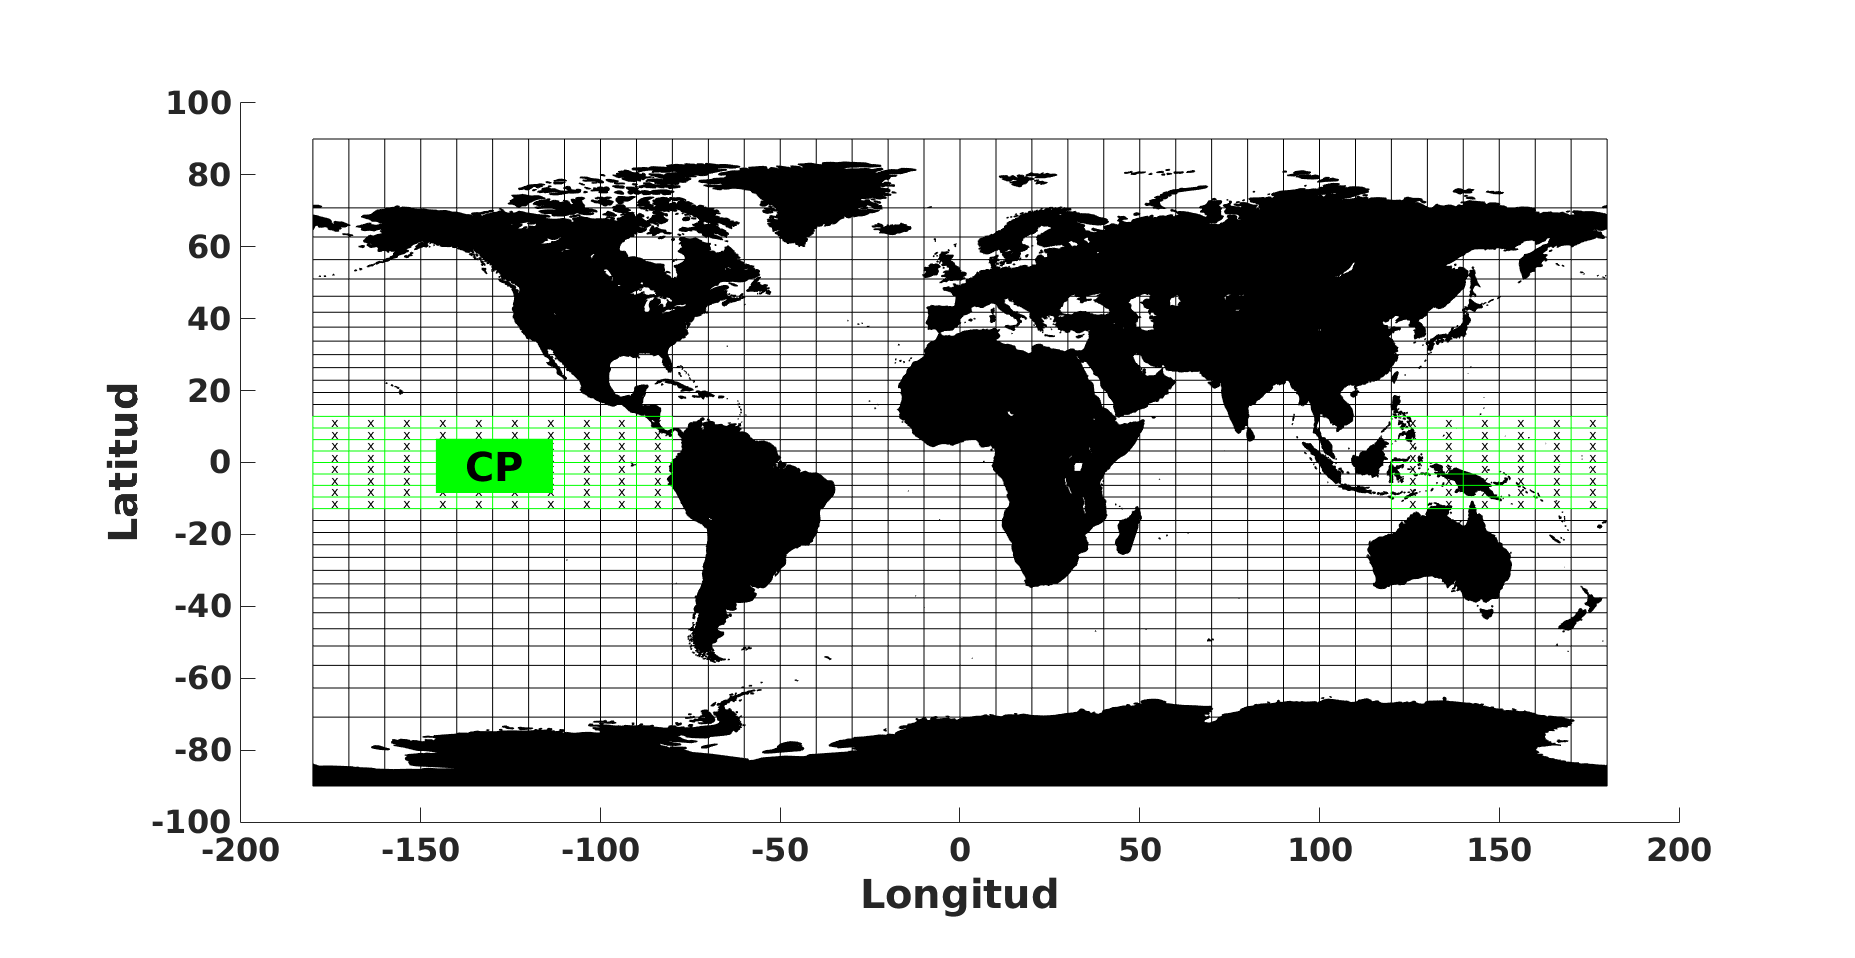
\includegraphics[width=0.8\textwidth]{mapa3_2_CP.png}
 \caption[Figura región del Pacífico Central]{Mapa global, que muestra la región del Pacífico Central que fue aislada en la simulación cGENIE.}
  \label{fig:Mapa_CP}
\end{figure}
\newpage

\begin{table}[H]
\centering
\begin{tabular}{|c|c|c|c|c|}
\hline
& \multicolumn{4}{c|}{Reducci\'on de $pCO_2$ global} \\
\cline{2-5}
Modelo& Ajuste & Par\'ametros & R-cuadrado ($R^2$) & RMSE\\
\hline \hline
Lambert  & Logar\'itmico  & p1=-22.48, p2=533.5 y p3=3.261 & 1 & 0.0029 \\ \hline
%Albani & Logar\'itmico & p1=2.1 y p2=2.20$e^{-7}$& 0.998 & 0.06854\\ \hline
Takemura & Logar\'itmico & p1=-26.89, p2=631.4 y p3=4.256 & 0.9997 & 0.0165\\ \hline
MIROC-ESM & Logar\'itmico & p1=-33.13, p2=1011 y p3=5.237 & 0.9986 & 0.0518\\ \hline
MRI-CGCM3 & Logar\'itmico & p1=-15.38, p2=180.5 y p3=2.74 & 0.9999 & 0.0028\\ \hline
\end{tabular}
\caption[Coeficientes de ajuste CP]{Caracter\'isticas de los ajustes realizados a las reducciones globales de $pCO_2$, a partir de los resultados del modelo cGENIE. El ajuste general es logar\'itmico, 
su ecuaci\'on est\'andar es: $ f(x)=p1 + \frac{p2}{x} + p3*log(x)$. Donde f(x) es la reducci\'on de $pCO_2$ y x, el flujo de polvo de cada nivel para la zona del Pacífico central.}
\label{tabla:Res3}
\end{table}

Los valores de reducción de pCO$_2$ en esta zona son en general bajos y similares. El comportamiento de la simulación es descrita por una función logarítmica. La corta distancia entre los campos de polvo del Holoceno y UMG en cada una de los casos hacen que esta reducción sea similar a una función lineal.  

El mayor aporte es mostrado por la simulación MIROC-ESM ($\sim 3.6$ ppm). No obstante, la simulación Lambert casi triplica el campo de polvo de MIROC-ESM y dobla el aporte de Takemura en todos los niveles. La razón por la cual no se aprecia el aporte de los grandes flujos de polvo de Lambert, es debido a su alta variabilidad en esta zona. La razón de polvo Lambert entre el UMG y Holoceno varía entre -0.2 y 1.8 respectivamente (ver Anexos \ref{fig:L}), con valores positivos reflejando mayor presencia de polvo en el Último máximo Glacial que en el Holoceno, y valores negativos el caso inverso. Lo anterior es reflejado en una captura de $\sim 2.4$ ppm, ligeramente menor que la efectuada por el modelo Takemura ($\sim 2.6$ ppm) que posee una tasa entre -0.1 y 0.5. MIROC-ESM posee tasas de depositanción que varían entre 0 y 0.6 (mostrando un persistente incremento de flujos de polvo entre el Holoceno y UMG).  \newpage

 \begin{figure}[H]
        \begin{subfigure}[b]{0.5\textwidth}
                \includegraphics[width=\linewidth]{../../Figuras/Regionales/Albani/CP}
                \caption{Albani}
                \label{fig:L_R_CP}
        \end{subfigure}%
        \begin{subfigure}[b]{0.5\textwidth}
                \includegraphics[width=\linewidth]{../../Figuras/Regionales/Lambert/CP}
                \caption{Lambert}
                \label{fig:A_R_CP}
        \end{subfigure}%
        
        \begin{subfigure}[b]{0.5\textwidth}
                \includegraphics[width=\linewidth]{../../Figuras/Regionales/Takemura/CP}
                \caption{Takemura}
                \label{fig:T_R_CP}
        \end{subfigure}%
        \begin{subfigure}[b]{0.5\textwidth}
                \includegraphics[width=\linewidth]{../../Figuras/Regionales/MIROC-ESM/CP_log}
                \caption{MIROC-ESM}
                \label{fig:MI_R_CP}
        \end{subfigure}
        
        \begin{subfigure}[b]{0.5\textwidth}
                \includegraphics[width=\linewidth]{../../Figuras/Regionales/MRI-CGCM3/CP}
                \caption{MRI-CGCM3}
                \label{fig:MR_R_CP}
        \end{subfigure}
        \caption[Series de reducci\'on de $pCO_2$ de flujos regionales de polvo (CP)]{Reducci\'on de $pCO_2$ obtenidos mediante simulaci\'on cGENIE, para flujos de polvo cambiantes en la zona del Pacífico Central (CP) desde el Holoceno hasta el \'Ultimo M\'aximo Glacial.}\label{fig:CP}
\end{figure}

 El modelo MRI-CGCM3, posee los valores de flujo de polvo más bajos en todos los niveles desde el Holoceno hasta el Último Máximo Glacial (figura \ref{fig:MRI}). Esto se ve reflejado en su baja participación en la reducción de pCO$_2$ en esta región, no superando los $\sim 0.8$ ppm. 

Por otro lado, los campos de polvo de Albani presentan un alta variabilidad en sus tasas de depositación en la región CP. La mayor parte de la región tiene menores valores de polvo Albani durante el UMG que durante el Holoceno, que se refleja tanto en los valores de amplitudes que van desde -0.4 a 0.2 (\ref{fig:A}), como en los niveles de campos de polvo (figura \ref{fig:Albani}). Por lo anterior, la interpolación de los datos en esta zona produjo decrecimiento de polvo en gran parte del CP, pero al mismo tiempo enormes diferencias positivas de polvo (UMG-Holoceno), que se tradujo en una simulación no consistente. 

\subsection{Pac\'ifico Sur}

\begin{figure}[H]
\centering
 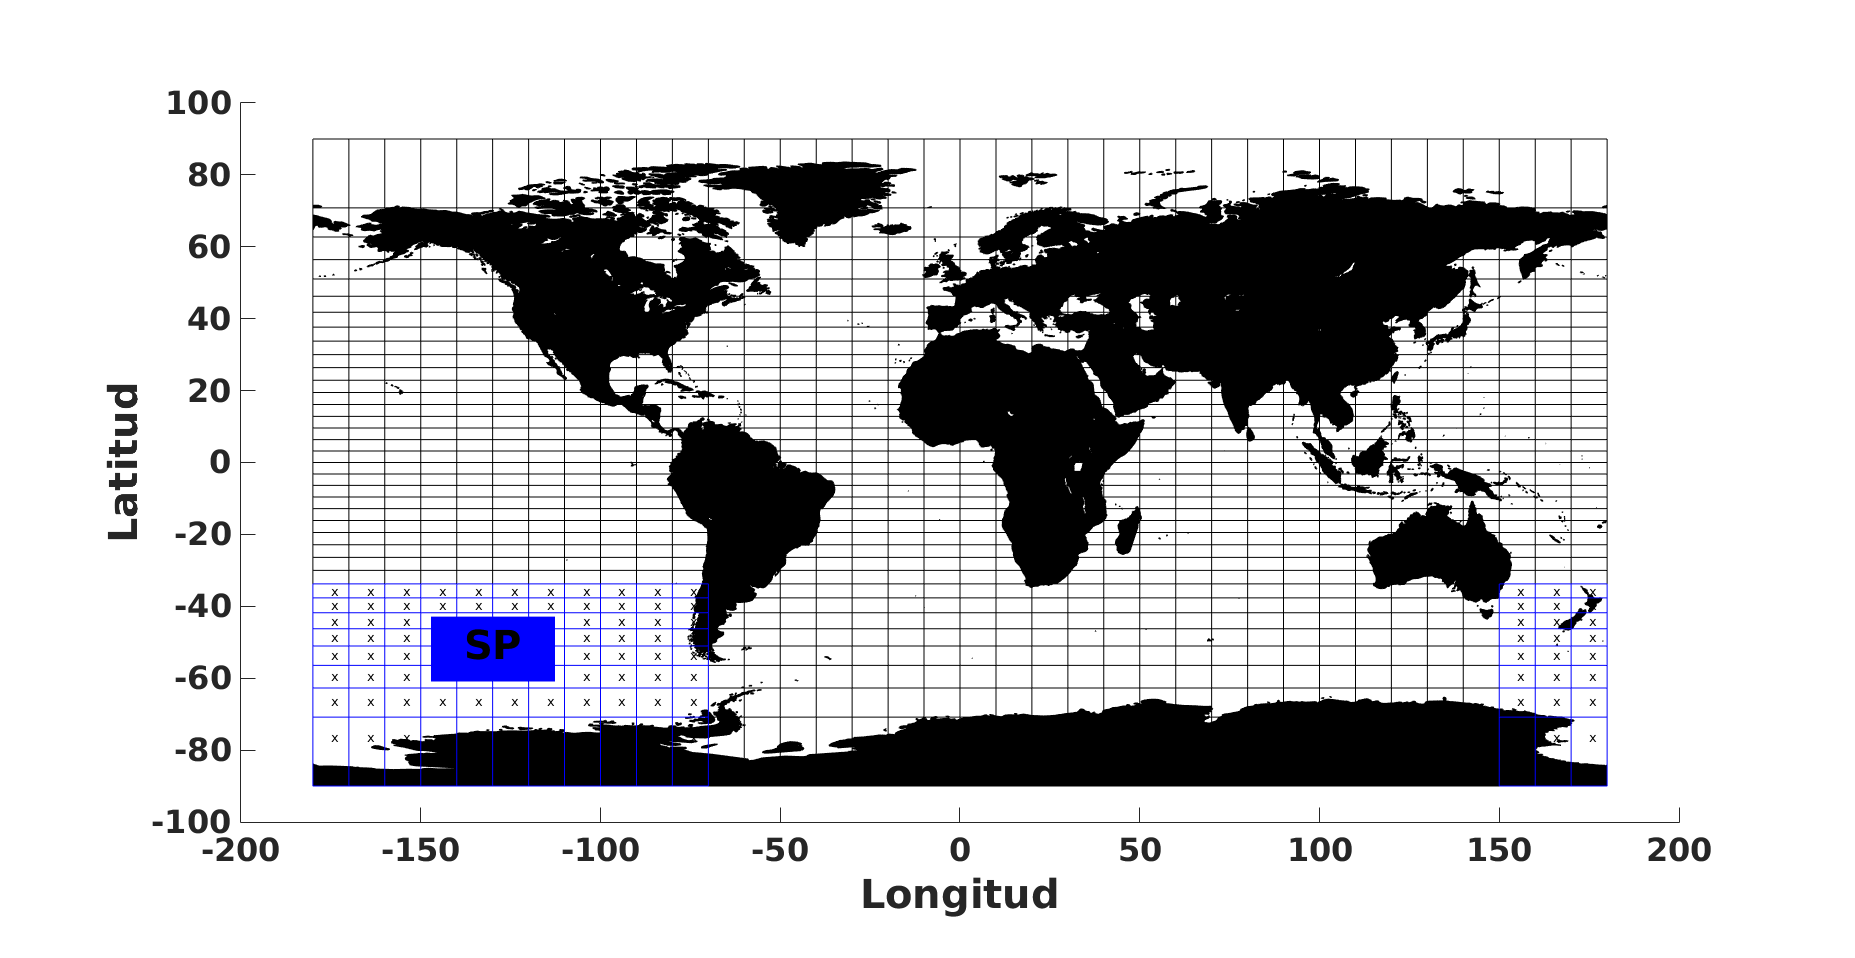
\includegraphics[width=0.8\textwidth]{mapa3_2_SP.png}
 \caption[Figura de región del Pacífico Sur]{Mapa global, que muestra la región del Pacífico Sur que fue aislada en la simulación cGENIE.}
  \label{fig:Mapa_SP}
\end{figure}

\begin{table}[H]
\centering
\begin{tabular}{|c|c|c|c|c|}
\hline
& \multicolumn{4}{c|}{Reducci\'on de $pCO_2$ global} \\
\cline{2-5}
Modelo& Ajuste & Par\'ametros & R-cuadrado ($R^2$) & RMSE\\
\hline \hline
Lambert  & Logar\'itmico  & p1=-22.48, p2=533.5 y p3=3.261 & 1 & 0.0029 \\ \hline
Albani & Logar\'itmico & p1=-457.4, p2=3.241e+04 y p3=63.2 &  0.38 & 0.2088\\ \hline
Takemura & Logar\'itmico & p1=45.27, p2=-816.4 y p3=-8.036 & 0.9982 & 8.0717e-04 \\ \hline
%MIROC-ESM & Lineal & p1=1.23$e^{-13}$ y p2=-1.03 & 0.9942 & 0.06412\\ \hline
%MRI-CGCM3 & Lineal & p1=1.60$e^{-13}$ y p2=-0.99 & 0.9876 & 0.01904\\ \hline
\end{tabular}
\caption[Coeficientes de ajustes SP]{Caracter\'isticas de los ajustes realizados a las reducciones globales de $pCO_2$, a partir de los resultados del modelo cGENIE. El ajuste general es logar\'itmico, 
su ecuaci\'on est\'andar es: $ f(x)=p1 + \frac{p2}{x} + p3*log(x)$. Donde f(x) es la reducci\'on de $pCO_2$ y x, el flujo de polvo de cada nivel para la zona del Pacífico Sur.}
\label{tabla:Res4}
\end{table} \newpage

 \begin{figure}[H]
        \begin{subfigure}[b]{0.5\textwidth}
                \includegraphics[width=\linewidth]{../../Figuras/Regionales/Albani/SP}
                \caption{Albani}
                \label{fig:L_R_SP}
        \end{subfigure}%
        \begin{subfigure}[b]{0.5\textwidth}
                \includegraphics[width=\linewidth]{../../Figuras/Regionales/Lambert/SP}
                \caption{Lambert}
                \label{fig:A_R_SP}
        \end{subfigure}%
        
        \begin{subfigure}[b]{0.5\textwidth}
                \includegraphics[width=\linewidth]{../../Figuras/Regionales/Takemura/SP}
                \caption{Takemura}
                \label{fig:T_R_SP}
        \end{subfigure}%
        \begin{subfigure}[b]{0.5\textwidth}
                \includegraphics[width=\linewidth]{../../Figuras/Regionales/MIROC-ESM/SP}
                \caption{MIROC-ESM}
                \label{fig:MI_R_SP}
        \end{subfigure}
        
        \begin{subfigure}[b]{0.5\textwidth}
                \includegraphics[width=\linewidth]{../../Figuras/Regionales/MRI-CGCM3/SP}
                \caption{MRI-CGCM3}
                \label{fig:MR_R_SP}
        \end{subfigure}
        \caption[Series de reducci\'on de $pCO_2$ de flujos regionales de polvo (SP)]{Reducci\'on de $pCO_2$ obtenidos mediante simulaci\'on cGENIE, para flujos de polvo cambiantes en la zona del Pacífico Sur (SP) desde el Holoceno hasta el \'Ultimo M\'aximo Glacial.}\label{fig:SP}
\end{figure}

El caso Lambert posee los mayores niveles de depositación de polvo en estas latitudes (ver imagen \ref{fig:Mapa_Lambert}). Ésto se refleja en un máximo de reducción de pCO$_2$ de $\sim 4.6$ ppm. No obstante, si bien Albani posee magnitudes de polvo $\sim 5$ veces inferiores en cada nivel comparado con Lambert, tiene una reducción de pCO$_2$ de $\sim 3$ ppm. Ésto, se encuentra asociado a la menor variabilidad de amplitudes UMG:Holoceno (entre $\sim 0.8$ y $1.6$, figura \ref{fig:A}) en comparación a Lambert (entre -0.2 y 1.2) (ver anexo \ref{fig:L}). 

El modelo Takemura, muestra un ínfima reducción de $\sim 0.04$ ppm para el UMG, lo que refleja poco aporte de polvo en estas latitudes (ver \ref{fig:Takemura}). MIROC-ESM y MRI-CGCM3 son modelos que no poseen fuentes de polvo en estas latitudes, por ende, muestra una progresiva disminución de flujo de polvo desde el Holoceno hasta el UMG. El caso más crítico es mostrado por el modelo MIROC-ESM con amplitudes UMG:Holoceno entre -0.4 y 0 (ver Anexo \ref{fig:MI}).   

\subsection{Atl\'antico Sur}

\begin{figure}[H]
\centering
 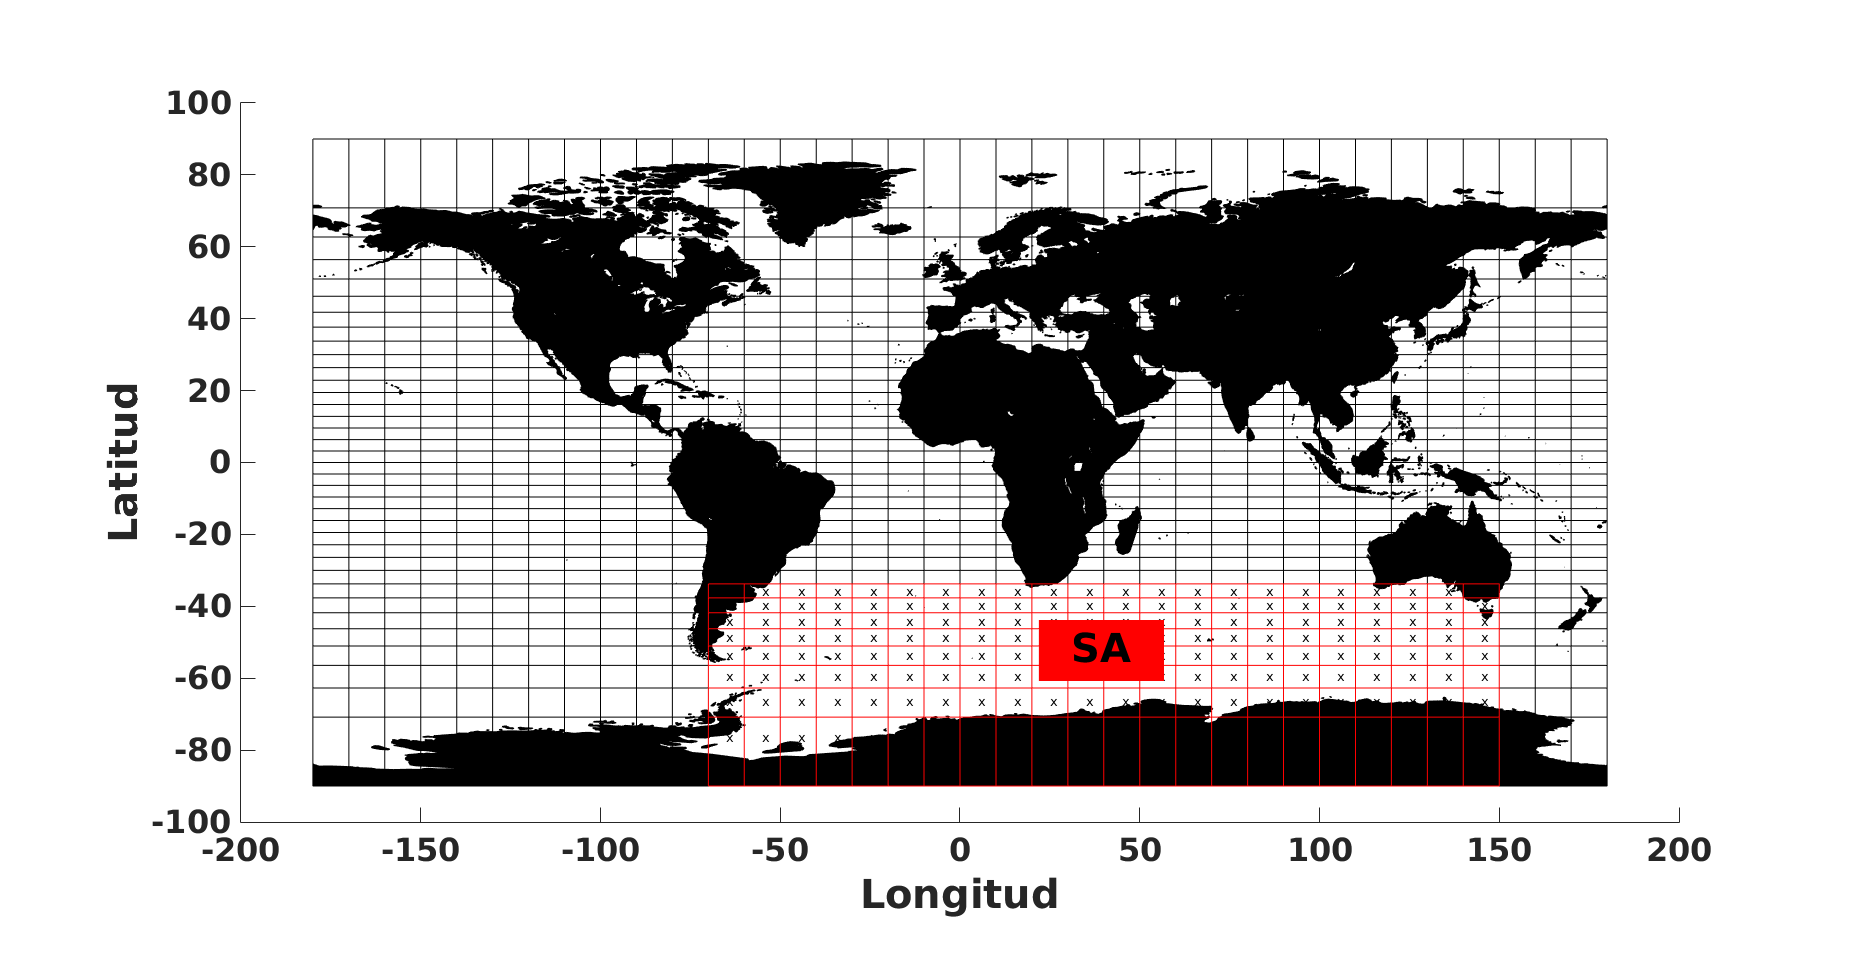
\includegraphics[width=0.8\textwidth]{mapa3_2_SA.png}
 \caption[Figura región del Atlántico Sur]{Mapa global, que muestra la región del Atlántico Sur que fue aislada en la simulación cGENIE.}
  \label{fig:Mapa_SA}
\end{figure}

\begin{table}[H]
\centering
\begin{tabular}{|c|c|c|c|c|}
\hline
& \multicolumn{4}{c|}{Reducci\'on de $pCO_2$ global} \\
\cline{2-5}
Modelo& Ajuste & Par\'ametros & R-cuadrado ($R^2$) & RMSE\\
\hline \hline
Lambert  & Logar\'itmico  & p1=-69.08, p2=1.47e+04 y p3=8.09 & 0.9986 & 0.0808 \\ \hline
Albani & Logar\'itmico & p1=-18.92, p2=-72.4 y p3=3.116 & 0.9993 & 0.1232\\ \hline
%Takemura & Lineal & p1=1.14$e^{-13}$ y p2=-1.3 & 0.9966 & 0.03623\\ \hline
%MIROC-ESM & Lineal & p1=1.23$e^{-13}$ y p2=-1.03 & 0.9942 & 0.06412\\ \hline
MRI-CGCM3 & Logar\'itmico & p1=-26.43, p2=1258 y p3=3.492 & 0.9999 & 0.01040\\ \hline
\end{tabular}
\caption[Coeficientes ajuste SA]{Caracter\'isticas de los ajustes realizados a las reducciones globales de $pCO_2$, a partir de los resultados del modelo cGENIE. El ajuste general es logar\'itmico, 
su ecuaci\'on est\'andar es: $ f(x)=p1 + \frac{p2}{x} + p3*log(x)$. Donde f(x) es la reducci\'on de $pCO_2$ y x, el flujo de polvo de cada nivel para la zona del Atlántico sur. }
\label{tabla:Res5}
\end{table}

 \begin{figure}[H]
        \begin{subfigure}[b]{0.5\textwidth}
                \includegraphics[width=\linewidth]{../../Figuras/Regionales/Albani/SA}
                \caption{Albani}
                \label{fig:L_R_SA}
        \end{subfigure}%
        \begin{subfigure}[b]{0.5\textwidth}
                \includegraphics[width=\linewidth]{../../Figuras/Regionales/Lambert/SA_log}
                \caption{Lambert}
                \label{fig:A_R_SA}
        \end{subfigure}%
        
        \begin{subfigure}[b]{0.5\textwidth}
                \includegraphics[width=\linewidth]{../../Figuras/Regionales/Takemura/SA}
                \caption{Takemura}
                \label{fig:T_R_SA}
        \end{subfigure}%
        \begin{subfigure}[b]{0.5\textwidth}
                \includegraphics[width=\linewidth]{../../Figuras/Regionales/MIROC-ESM/SA}
                \caption{MIROC-ESM}
                \label{fig:MI_R_SA}
        \end{subfigure}
        
        \begin{subfigure}[b]{0.5\textwidth}
                \includegraphics[width=\linewidth]{../../Figuras/Regionales/MRI-CGCM3/SA}
                \caption{MRI-CGCM3}
                \label{fig:MR_R_SA}
        \end{subfigure}
        \caption[Series de reducci\'on de $pCO_2$ de flujos regionales de polvo (SA)]{Reducci\'on de $pCO_2$ obtenidos mediante simulaci\'on cGENIE, para flujos de polvo cambiantes en la zona del Atlántico Sur (SA) desde el Holoceno hasta el \'Ultimo M\'aximo Glacial.}\label{fig:SA}
\end{figure}

La simulación de Albani, tiene la mayor reducción de pCO$_2$ estimada para el UMG ($\sim 12.5$ ppm). La figura \ref{fig:Albani}, muestra la existencia de una intensa fuente de polvo localizada en América del Sur, en las cercanías de la Patagonia chileno-argentina. Esto explica las altas tasas de depositación de polvo en relación a los otros casos (la amplitud UMG:Holoceno alcanza valores entre 1.2-1.4). 

La reconstrucción Lambert con también una fuente de polvo en la zona Pagónica de Sur América, aunque con valores inferiores a los estimados por Albani, y con más estrechas diferencias entre el Holoceno y UMG, tienen una disminución de pCO$_2$ de $\sim 6$ ppm. A su vez, MRI-CGCM3 posee una muy pequeña fuente de polvo en la misma zona (ver figura \ref{fig:MRI}), lo que se traduce en que los flujos de polvo produzcan una disminución de pCO$_2$ de $\sim 1$ ppm. En relación a Takemura y MIROC-ESM, ambos no poseen fuentes de polvo en la zona cercana al Atlántico Sur, por ende, en ambos casos el modelo cGENIE simula una progresiva liberación de CO$_2$ desde el océano hacia la atmósfera, alcanzado valores de -0.49 y -1.22 ppm desde el Holoceno al UMG respectivamente. 


\section{Resultados finales}

\begin{figure}[H]
\centering
 \includegraphics[width=0.85\textwidth]{../../Figuras/Ponderaciones/Ponderaciones_LGM}
 \caption[Contribución ponderada de las zonas HNLC a la reducción de CO$_2$ global]{Contribución ponderada de las zonas HNLC (Atlántico Sur, Pacífico Sur, Pacífico Norte y Pacífico Central) a la reducción de pCO$_2$ global. En rojo las contribución relativa del modelo Albani, en verde la correspondiente a la reconstrucción Lambert, en morado la contribución Takemura, en rosado el aporte de MIROC-ESM y en negro la participación de MRI-CGCM3.   }
  \label{fig:Ponderacion}
\end{figure}

En la figura \ref{fig:Ponderacion} sólo se consideraron las simulaciones que reflejaban un incremento en los campos de polvo y, por lo tanto, un progresivo aumento en la captación de pCO$_2$ por parte de las distintas regiones oceánicas (SA, SP, NP, CP), en relación a su reducción total. 

En concordancia con los resultados regionales, vemos que las respuesta de los distintos casos y sus respectivos flujos de polvo en la región CP, tiene un menor aporte a la reducción total en cualquiera de las simulaciones. Sin embargo, vemos también que los campos de polvo en esta latitud son menores en relación a otras zonas en todos los casos (ver figuras del UMG en el capítulo 4 y \ref{fig:MR}). Además que la zona muestra en general un gradiente zonal de depositación, con mayores flujos en la zona este del Pacifico y menor en la zona oeste. No obstante, esta región presenta un buen ajuste de las simulaciones quedando rezagado sólo el modelo MRI-CGCM3, el cual como vimos es el que menor captación tiene en el área ($\sim 0.8$ ppm) para un total de $\sim 9$ ppm producto de la mínima presencia de flujo de polvo registrada por el modelo en cada nivel del periodo de estudio (ver figura \ref{fig:MRI}). Así la media de reducción de pCO$_2$ calculada entre las distintas simulaciones se encuentra en torno a los 2.4 ppm, es decir, un $\sim 15\%$ de aporte en la captura de esta región oceánica. 


La región del Pacífico Norte, muestra un buen acuerdo entre los modelos en torno a la mayor participación de la región en la reducción de pCO$_2$ global ($\sim 30\% $), a pesar de la alta variabilidad en los flujos de polvo. La zona NP tiene una media de $\sim 5$ ppm. Lo que implica que los modelos de polvo presentan un intrusión importante de flujo en el área, cuya sensibilidad producto de la depositación es alta y se ve reflejado en la biogeoquímica de la productividad biológica establecida en cGENIE. El modelo Takemura, no presenta fuente de polvo en las cercanías de esta zona (ver figura \ref{fig:Takemura}). 

Por otro lado, la región SP con una media de $\sim 1.55$ ppm, representa una contribución del $\sim 14\%$. Sin embargo, vemos que la variabilidad de las reducciones entre los distintos casos depende de la intensidad y de la ubicación de la fuente de polvo para esta zona. Dado que los modelos muestra grandes diferencias en los flujos de polvo, no se puede asegurar el porcentaje de participación en la captura de pCO$_2$, pero si se puede afirmar que en presencia de una fuente de polvo, esta zona oceánica responderá en su biología al eventual suministro de hierro. 

La región SA muestra ser la que más aporta en la captura de pCO$_2$, rangeando entre $\sim 11\%$ para valores bajos de suministro de polvo y $\sim 58\%$ para suministro mayores (con una media de $\sim 34\%$). Si bien, no hay un buen ajuste entre los modelos en torno a la cantidad de polvo en los distintos niveles y en particular para el UMG, si se ve que existe una alta sensibilidad a la magnitud del suministro en esta región oceánica, y que será la que mayor captura realice (Lambert tiene el doble de flujo de polvo en NP que en SA, sus capturas respectivamente son $\sim 5$ p.p.m. y $\sim 6$ ppm). 

Finalmente, vemos que la reconstrucción Lambert, posee una buena asimilación por parte del modelo cGENIE en todas las simulaciones, además que guarda cierta prudencia en cada una de sus estimaciones. No obstante, posee una gran variabilidad que no es capturada por otros modelos de flujos de polvo vistos en este trabajo. Por ende, se requieren mayores comparaciones para darle un mayor grado de confianza. Por otro lado, el modelo MIROC-ESM es el que muestra menos presencia en las simulaciones, debido su escasa existencia de fuentes en el Hemisferio Sur, además parece tener una drástica respuesta en sus estimaciones para distintas zonas, por ende, parece ser el modelo más débil en esta investigación. Los campos de polvo MRI-CGCM3 han resultado hasta ahora, las simulaciones más reservadas de captura de pCO$_2$. 

\chapter{Consideraciones finales}

% !TEX root = ../Tesis_NataliaOpazo.tex


La depositación de polvo aéreo es una fuente importante de hierro para el oc\'eano, particularmente en las zonas HNLC \citep{jin2008impact,martinez2014iron,lambert2015dust}. \'Esto dato que ejerce un control en la biología marina por su baja concentración, convirtiéndose en un elemento limitante \citep{falkowski1998biogeochemical,martin1990glacial,gruber2008marine,tagliabue2017integral}.

El incremento de flujos de polvo durante periodos glaciares \citep{mahowald1999dust,gaspari2006atmospheric,lambert2008dust,maher2010global,lamy2014increased} pudo haber estimulado la productividad primaria y/o la producción de exportación de materia orgánica, por lo que puede ser un factor determinante en la diferencia entre 80 y 100 ppm \citep{sigman2000glacial,hain2010carbon,ferrari2014antarctic} de concentración atmosférica de CO$_2$ durante periodo glaciares e interglaciares.

Con el propósito de evaluar la sensibilidad de la bomba biológica al suministro de hierro y cómo este afecta la concentración de pCO$_2$ atmosférico, es que realizó una prueba mediante el modelo biogeoquímico de complejidad intermedia cGENIE durante el periodo que abarca desde el UMG y el comienzo del Holoceno, a partir, de cinco campos de flujos de polvo \citep{lambert2015dust,yukimoto2012new,sueyoshi2013set,takemura2009simulation,albani2014improved} provenientes tanto de modelos como de recontrucciones. Obteniéndose un promedio máximo de reducción de pCO$_2$ a nivel global en torno a los 17 ppm. Valor que está ligeramente por sobre lo estimado por otros trabajos desarrollado por medio de modelos GCM más complejos como PISCES y los desarrollados por MIT, a partir de los cuales se estima una captura por parte de los océanos correspondiente a aproximadamente 8 \citep{parekh2006atmospheric,lambert2015dust}, 11 \citep{tagliabue2009quantifying} y 15 ppm \citep{bopp2003dust}. Por otro lado, modelos de caja como \cite{hain2010carbon} estima una captura de alrededor de 35 ppm, valor que está muy por sobre los máximos 21 ppm evaluados por medio de los flujos de polvo desarrollados por \cite{albani2014improved}. 

Estos resultados estarían reflejando que la mayor liberación de polvo sobres los océanos superficiales durante el LGM habría permitido mejorar la utilización de NO$_{3}^{-}$ y PO$_{4}^{3-}$, debido a un aumento en la disponibilidad de hierro. Macro y micronutrientes que en conjunto con el CO$_2$ disuelto forman parte del fitoplancton lo que permitiría dicha disminución en la concentración atmosférica de CO$_2$.

Cálculos de los aportes regionales en la captura de pCO$_2$ muestran que son las altas latitudes (Océanos del Sur y Pacífico Norte) las que mayor control ejercen sobre la variabilidad de este gas, lo que se corresponde con lo mostrado por \cite{lambert2015dust} y \cite{bopp2003dust}. 

Si bien es sabido que en regiones subpolares como los Océanos del Sur, aguas profundas afloran llevando grandes contenidos de nutrientes a las superficies en estas regiones. Proceso que podría producir una liberación de CO$_2$ hacia la atmósfera, además de un gran suministro de nutrientes que en la actualidad es rápidamente devuelto a las profundidades del océanos sin lograr ser utilizados para la formación de biomasa \citep{hain2010carbon}. La mayor captura durante el UMG podría deberse, por un lado, a que hubo un aumento en la cobertura de hielo en la zona Antártica \citep{ferrari2014antarctic}, lo que habría generado un bloqueo y eventual desplazamiento de gran parte de la surgencia de agua profunda hacia el océano subtropical, conllevando a un menor suministro de CO$_2$ (evitando una liberación de éste desde las aguas oceánicas superficiales hacia la atmósfera), y por otro lado, un menor suministro de nutrientes \citep{tagliabue2009quantifying} que habría sido mejor utilizado debido a la mayor tasa de polvo durante este periodo, que habría mejorado la fertilización con hierro a los océanos provocando un aumento del flujo de PE \citep{martin1990glacial,toggweiler2006midlatitude,shaffer2018and}. 

 Además en las zonas HNLC limitadas por hierro existe una predominancia de diatomeas \citep{bopp2003dust,arellano2011high} para las cuales la concentración de Si(OH)$_4$ es limitante. Por esta razón, se ha propuesto que durante el UMG la mayor utilización de NO$_{3}^{-}$ y PO$_{4}^{3-}$ por otros organismo planctónicos podría haber dejado un excedente de Si(OH)$_4$ que producto de la circulación marina podría haber sido transportado a zonas con limitación de Si(OH)$_4$ como las regiones subtropicales de giros oligotróficos, provocando una captura general mayor de pCO$_2$ atmosférico entre el UMG y el Holoceno \citep{matsumoto2002silicic}, sin embargo, hay estudios que se contraponen a esta idea como \cite{tagliabue2014impact} que muestra que una mayor deposición de hierro en altas latitudes, provoca una disminución de Si producto de una mayor utilización, generando un menor transporte a bajas latitudes. 

Los resultados presentados, son valores que están sujetos a la variabilidad inducida por los propios modelos de polvo utilizados como forzantes, en este caso mediante cGENIE, los cuales sobrestiman en la mayoría de los casos los niveles de depositación de polvo en latitudes del norte y subestiman las fuentes glaciogénicas del hemisferio sur durante el LGM, razón por la cual este trabajo es un primer acercamiento en torno al efecto del hierro proveniente de fuentes eólicas en la bomba biológica. No obstante, tanto la concentración de ligandos como la fuente de Fe son factores que pueden cambiar y que tienen una consecuencia en la PE. Finalmente, si bien vemos que la bomba biológica tiene un impacto en la reducción de CO$_2$ este efecto no alcanza a explicar toda la diferencia entre el UMG y el Holoceno, por lo tanto, otros factores como la alcalinidad del océano, la bomba de carbonato y/o mecanismo físicos como la estratificaci\'on pueden estar actuando para explicar esta variabilidad.  

Las dos hipótesis planteadas en este trabajo son aceptadas (H$_{0}$), dado que ambas se cumplen. Como vimos, existe un efecto del polvo en el $\Delta$pCO$_{2}$ del periodo que abarca entre el UMG y el Holoceno. El $\Delta$pCO$_{2}$ generado proviene en su mayoría de los cambios en los océanos del sur. 





\bibliographystyle{apalike}
\bibliography{Citas2}
\pagenumbering{Roman}
\setcounter{page}{4}
\addcontentsline{toc}{chapter}{Bibliograf\'ia}

\chapter{Anexos}
\pagenumbering{Roman}
\setcounter{page}{5}
%\addcontentsline{toc}{chapter}{Anexos}
%\begin{quotation}
% !TEX root = ../Tesis_NataliaOpazo.tex 


\begin{figure}[H]
\centering
 \includegraphics[width=1.2\textwidth]{../../Figuras/Spin-up/Ingles/SPIN-UP}
 \caption[Simulación spin-up]{Serie de pCO$_2$ obtenidos a partir de las simulaciones spin-up realizadas mediante el modelo cGENIE, para el periodo que va desde el Holoceno hasta el UMG. La primera fila muestra la temperatura superficial, mientra la segunda fila presenta la temperatura de fondo para todos los casos.}
  \label{fig:SPIN-UP}
\end{figure}
\newpage

 \begin{figure}[H]
        \begin{subfigure}[b]{0.55\textwidth}
                \includegraphics[width=\linewidth]{../../Figuras/Amplitud/Albani_amplitud2.pdf}
                \caption{Lambert}
                \label{fig:L}
        \end{subfigure}%
        \begin{subfigure}[b]{0.55\textwidth}
                \includegraphics[width=\linewidth]{../../Figuras/Amplitud/Lambert_Amplitud2.pdf}
                \caption{Albani}
                \label{fig:A}
        \end{subfigure}%
        
        \begin{subfigure}[b]{0.55\textwidth}
                \includegraphics[width=\linewidth]{../../Figuras/Amplitud/MIROC_Amplitud2.pdf}
                \caption{Takemura}
                \label{fig:T}
        \end{subfigure}%
        \begin{subfigure}[b]{0.55\textwidth}
                \includegraphics[width=\linewidth]{../../Figuras/Amplitud/MRI-CGCM3_Amplitud2.pdf}
                \caption{MIROC-ESM}
                \label{fig:MI}
        \end{subfigure}
        
        \begin{subfigure}[b]{0.55\textwidth}
                \includegraphics[width=\linewidth]{../../Figuras/Amplitud/Takemura_Amplitud2.pdf}
                \caption{MRI-CGCM3}
                \label{fig:MR}
        \end{subfigure}
        \caption[Amplitud flujos de polvo]{Diferencia de flujos de polvo entre el UMG y el Holoceno}\label{fig:Amp}
\end{figure}

\newpage

Este proceso es llevado a cabo con el fin de posterior a las corridas cGENIE, graficar los datos de CO$_2$ obtenidos con respecto a la masa de polvo que se deposita en una celda de las regiones HNLC cada año. Así, posteriormente sumamos los valores para una regi\'on y tenemos la masa total de polvo que se deposita por año en esta zona. 

Para obtener una fracci\'on de \'area de la tierra en funci\'on de una latitud y longitud determinada, vamos a considerar la tierra una esfera de tipo
  elipsoide (figura \ref{fig:mundo1_met}). Donde la ecuaci\'on \ref{eq:met2} nos permiti\'o obtener dicha \'area. 
  \begin{equation} \label{eq:met2}
   A_{sup}=\displaystyle\int_{\varphi_1}^{\varphi_2} R \left( \displaystyle\int_{\lambda_2}^{\lambda_2} R\ cos\varphi\ d\lambda \right) d\varphi = R^{2} 
  \left(\lambda_2 - \lambda_1 \right) \left(sen\varphi_2 - sen\varphi_1 \right) 
  \end{equation}
  
   Donde R es el radio de la tierra (apr\'oximadamente 6371 km); y donde\\
   $ 0\leqq \lambda_1 \leqq \lambda \leqq \lambda_2 \leqq 2\pi $ y donde, $ \frac{-\pi}{2} \leqq \varphi_1 \leqq \varphi \leqq \varphi_2 \leqq \frac{\pi}{2}$.
  
  \begin{figure}[H]
  \centering
  \includegraphics[width=0.3\textwidth]{mundo1_met.png}
  \caption[Área superficial de una grilla]{\'Area superficial de una celda de grilla entre longitudes $ \lambda_1\ y\ \lambda_2 $ y latitudes $ \varphi_1\ y\ \varphi_2$.}
  \label{fig:mundo1_met}
\end{figure}

 Para realizar el calculo anterior se ocupo una funci\'on MATLAB denomina \textit{areaquad} y los datos de longitud y latitud de cuadrantes especificados en
 la tabla \ref{tabla:Area1}. As\'i los resultados son expresado en unidades de metros cuadrados ($m^{2}$).

 \newpage

\begin{table}[H] 
\centering
\resizebox{16cm}{!} {%
\begin{tabular}{|ccc|}
\hline \hline
\multicolumn{3}{c}{\bf Configuración cGENIE} \\
%\cline{2}
\hline \hline
{\bf Componentes} & {\bf Prescripción} & {\bf Dato} \\
\hline \hline
CLIMA  & Retroalimentación  & Si\\ \hline
\multirow{4}{*}{\makecell{ESQUEMA DE PRODUCCIÓN \\ BIOLÓGICA NUEVA}} &
\makecell{Identificador de esquema \\ de exportación} & \makecell{$bio\_PFe$ (Plancton \\ no silíceo)} \\ \cline{2-3}
& Valor de saturación media PO4 & 0.10e$-6$ [mol kg$^{-1}$]\\ \cline{2-3}
& Valor de saturación media de Fe & 0.10E-09 [mol kg$^{-1}$]\\ \cline{2-3}
& \makecell{Escala de tiempo de absorción \\ de nutrientes  (por el plancton)} & 63.3827 \\ \hline
\makecell{TASA DE MATERIA ORGÁNICA \\ EXPORTADA} & \makecell{Fracción de producción de \\ materia orgánica disuelta} & 0.66 \\ \hline
\multirow{2}{*}{\makecell{TASA DE MATERIA INORGÁNICA\\ EXPORTADA}} & \makecell{Relación de exportación \\biológica CaCO3/POC}  & 0.0485 \\ \cline{2-3}
& {Estado de saturación ambiental} & 0.7440\\ \hline
\multirow{7}{*}{REMINERALIZACIÓN} & Tiempo de vida del DOC [años] & 1 \\ \cline{2-3}
& \makecell{Fraccionamiento de la \\ abundancia inicial del DOC} & 0.055 \\ \cline{2-3}
& \makecell{Profundidad de la remineralización\\ o POC}& 589.9451 \\ \cline{2-3}
& Longitud de la remineralización del POC & 1000000 \\ \cline{2-3}
& \makecell{Fraccionamiento de la \\ abundancia inicial del CACO3} & 0.45 \\ \cline{2-3}
& \makecell{Profundidad de la remineralización\\ o CACO3} & 1.8905e+3\\ \cline{2-3}
& Longitud de la remineralización del CaCO3 & 1000000\\ \hline
\multirow{11}{*}{HIERRO} & Solubilidad eólica & 0.00291468 \\ \cline{2-3}
& \makecell{Exponente de la solubilidad\\ del hierro} & \makecell{0.5 (1 en caso \\ de ser uniforme)}\\ \cline{2-3}
& \makecell{Modificador de la tasa de \\ eliminación de hierro disuelto} & \makecell{para el POC=1.338130\\
para el CaCO3=0; para el opalo=0\\
para el hierro=0}  \\ \cline{2-3} 
& Regeneración sin barrido & 0 \\ \cline{2-3}
& Retorno de POFe & No \\ \cline{2-3}
& Fe:C Variable & NO \\ \cline{2-3}
& Ajustar pk'(Fel) & 11 \\ \cline{2-3}
& \makecell{Máxima tasa de \\ materia orgánica} & 250000 \\ \cline{2-3}
& Tasa de dependencia Fe:C & \makecell{FetoC pP=-0.4225; \\
 FetoC K=103684; Fetoc C=0} \\ \hline
\multirow{2}{*}{FORZANTES} & Especificación de Forzante & Archivo base\_config \\ \cline{2-3}
& Concentración atmosférica de CO$_2$ & \makecell{278$e^{-6}$ (spin-up) o no \\ definido (simulaciones considerando el polvo)}  \\ \hline \hline 
\end{tabular}%
}
\caption[Configuración cGENIE]{Configuración ``User\_config'' del modelo cGENIE. } 
\label{tabla:U-conf}
\end{table} 


%\end{quotation}

\end{document}\grid
